%!TeX root=../main.tex

\chapter{Distribuzione e Prodotto finale}\label{ch:distribuzione-e-prodotto-finale}

\section{Strategia di distribuzione}\label{sec:strategia-di-distribuzione}
La fase di distribuzione ha avuto come obiettivo non solo il rilascio tecnico dell’applicazione, ma anche la validazione della sua utilizzabilità in un ambiente che simula condizioni reali di produzione.
Per \textbf{Swift Contest} è stato scelto un approccio multipiattaforma che copre i principali punti di accesso per i diversi tipi di utenti:
\begin{itemize}
    \item \textbf{Applicazione Web}: distribuita su \textbf{Vercel}, per garantire accessibilità universale da qualsiasi browser moderno, sia desktop che mobile.
    \item \textbf{Applicazione Android}: distribuita come pacchetto APK, reso disponibile tramite un meccanismo di download sicuro per un'esperienza d'uso ottimizzata su dispositivi mobili.
    \item \textbf{Infrastruttura Backend}: interamente gestita su \textbf{Supabase}, che ospita il database, lo storage, le funzioni serverless e i servizi realtime.
    \item \textbf{Pannello di Amministrazione}: sviluppato come strumento interno su \textbf{Retool} e interfacciato in modo sicuro con il backend, per le attività di moderazione e manutenzione.
\end{itemize}
Questa strategia ibrida consente di bilanciare la facilità di accesso (garantita dalla versione Web) con un'esperienza d'uso ottimizzata (offerta dalla versione Android), mantenendo al contempo un backend centralizzato, sicuro e scalabile.

\begin{figure}[H]
    \centering
    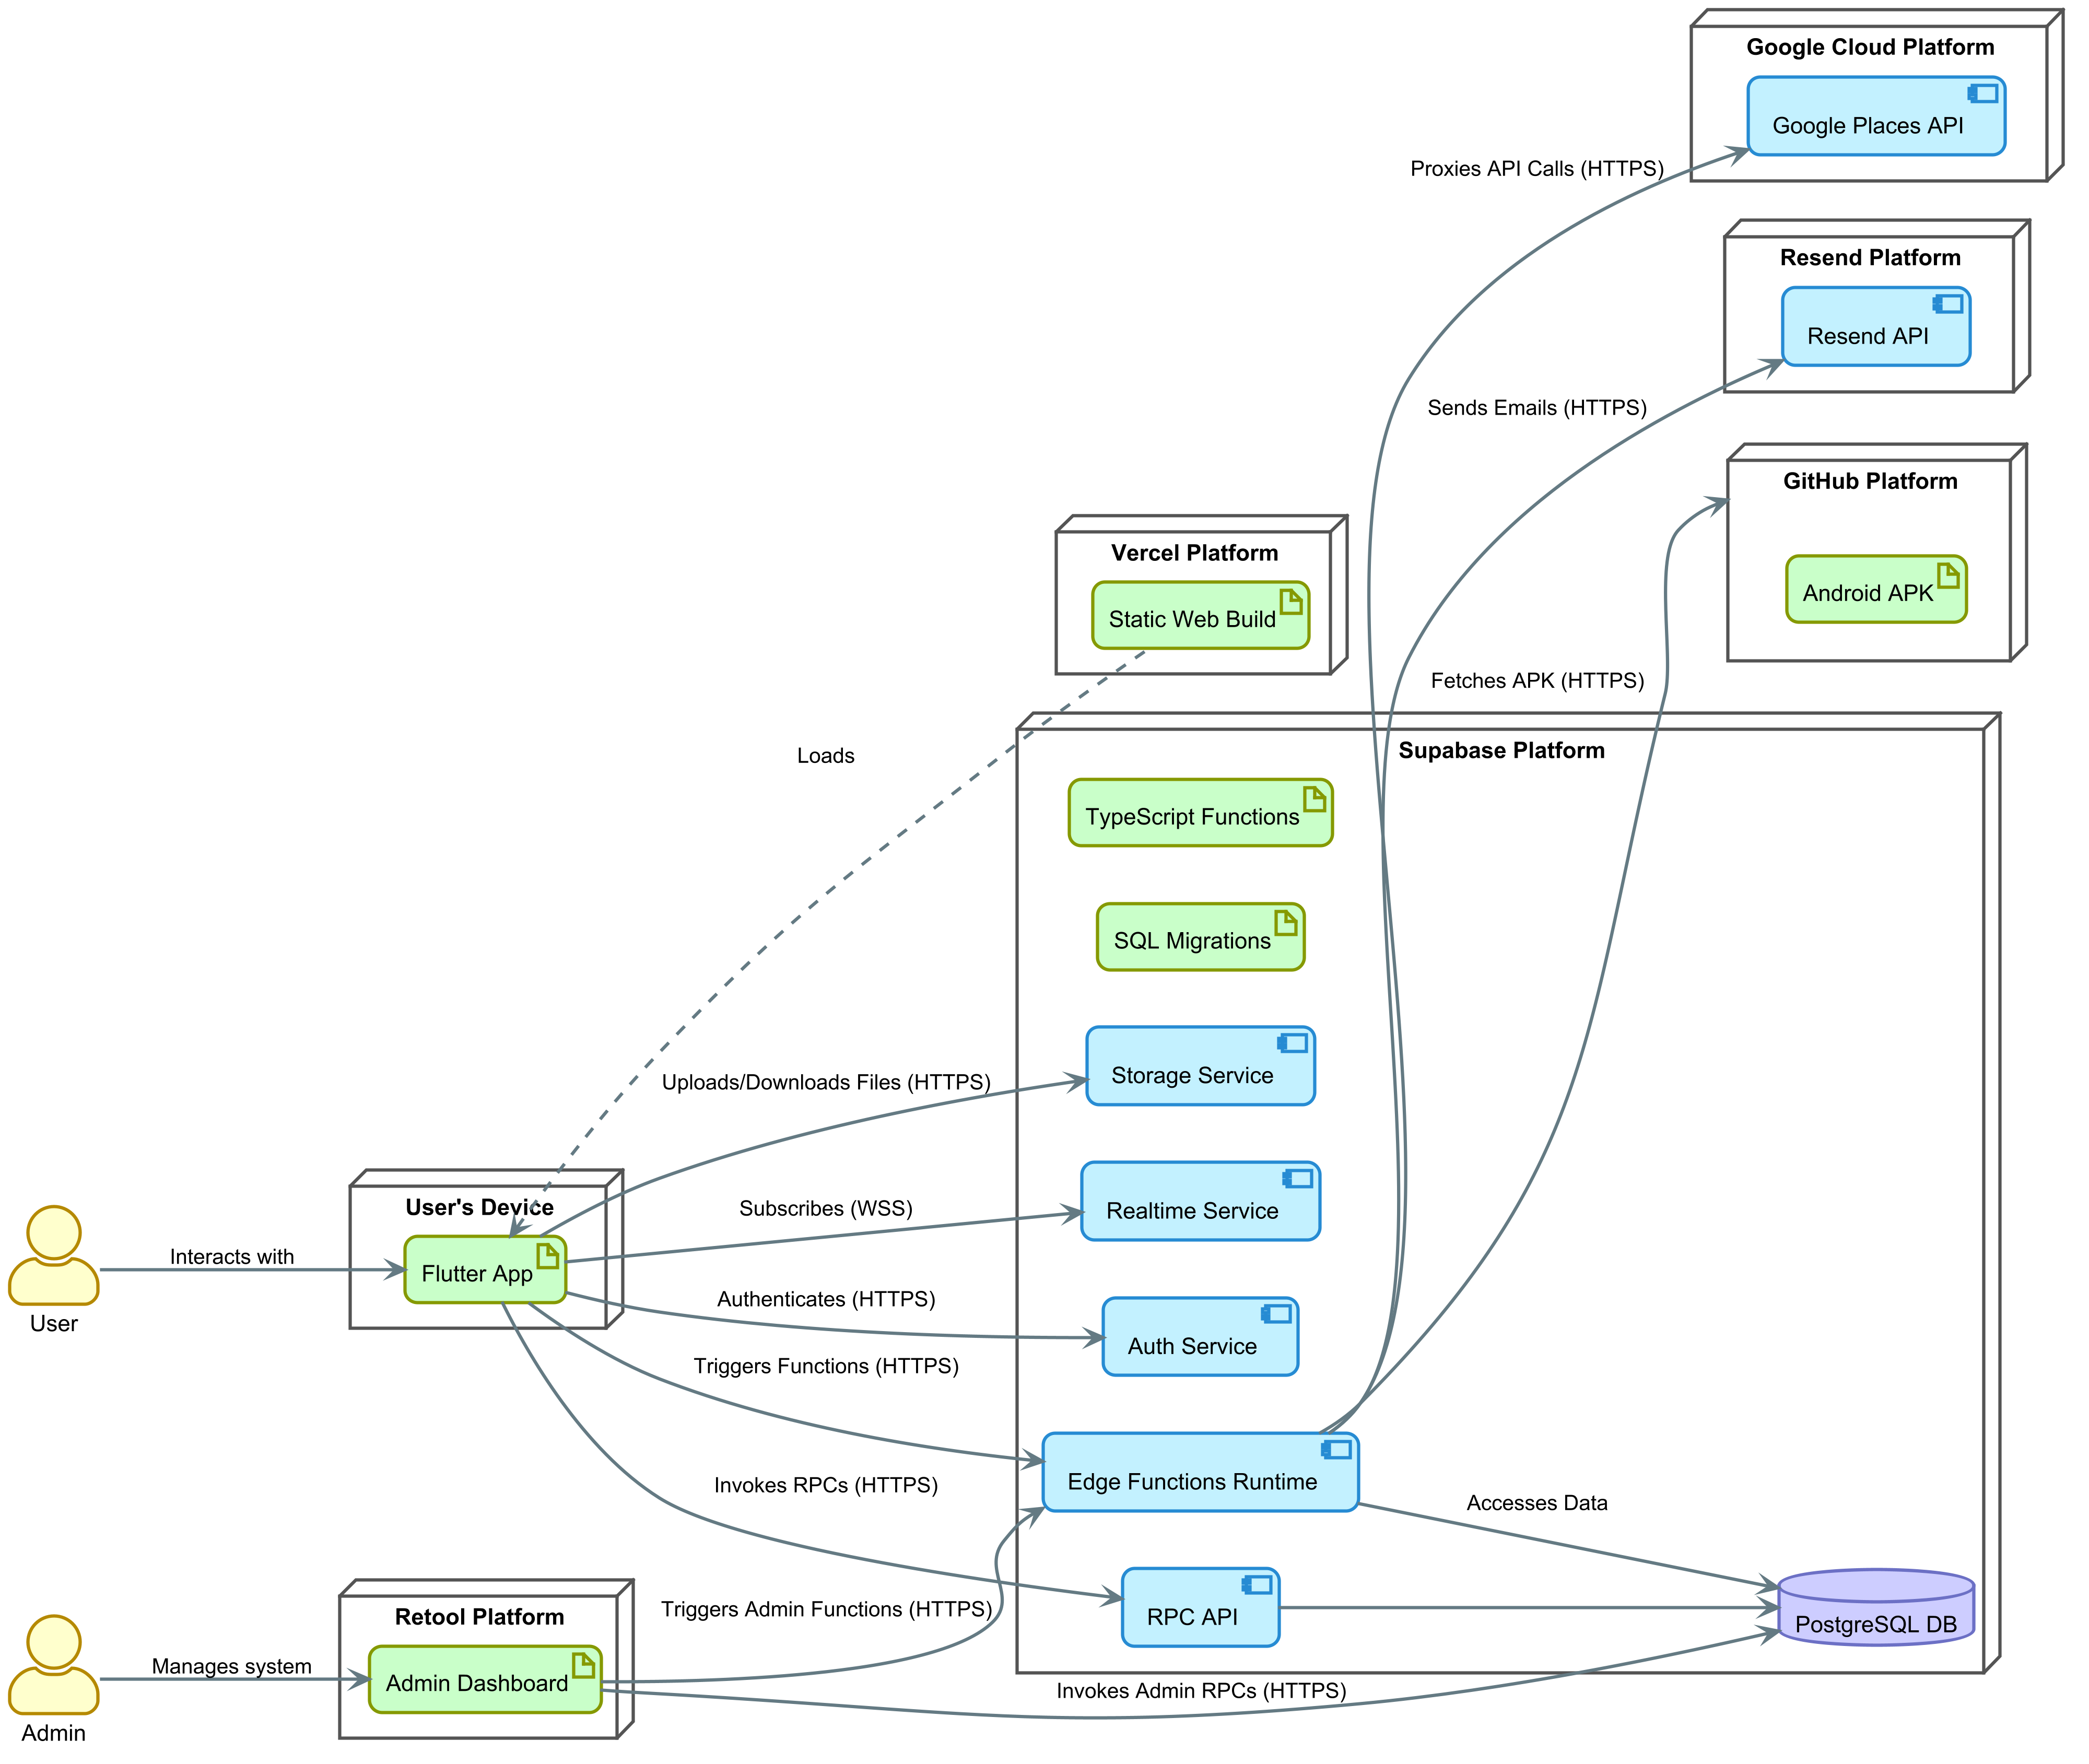
\includegraphics[width=\textwidth]{diagrams/deployment-diagram}
    \caption{Diagramma di Deployment dell'architettura completa di Swift Contest.}
    \label{fig:deployment_diagram}
\end{figure}

\section{Distribuzione Web su Vercel}\label{sec:distribuzione-web-su-vercel}
La versione Web dell'applicazione Flutter è stata distribuita su Vercel, una piattaforma serverless ottimizzata per la distribuzione di frontend moderni.
Il processo è completamente automatizzato tramite una pipeline di CI/CD (Continuous Integration/Continuous Deployment) integrata con il repository Git del progetto.
Ogni \emph{push} sul branch \texttt{main} innesca automaticamente una nuova build dell'applicazione Flutter in modalità \emph{release} e un conseguente deploy sulla piattaforma.

Per garantire il corretto funzionamento di una Single Page Application (SPA) come Flutter Web, è stato configurato un file \texttt{vercel.json} che gestisce il rewrite di tutte le rotte verso il file \texttt{index.html}, permettendo al router di Flutter (\texttt{auto\_route}) di gestire la navigazione lato client.

\section{Distribuzione Android}\label{sec:distribuzione-android}
Per la piattaforma Android, è stata prodotta una \textbf{release in formato APK}.
Data la natura prototipale del progetto, si è evitato il complesso processo di pubblicazione sul Google Play Store, optando per un approccio di distribuzione controllata che garantisce comunque sicurezza e facilità di aggiornamento:
\begin{enumerate}
    \item L'APK viene caricato come \emph{release asset} su un repository GitHub privato.
    \item Un'apposita Edge Function, \texttt{get-latest-apk}, è stata creata su Supabase per fungere da proxy sicuro.
    Questa funzione utilizza un Personal Access Token (PAT) di GitHub, memorizzato in modo sicuro in Supabase, per autenticarsi all'API di GitHub e scaricare l'asset.
    \item L'applicazione web offre un pulsante ``Download for Android'' che invoca questa Edge Function.
    L'utente riceve così l'ultima versione dell'APK direttamente dal backend, senza che il repository GitHub o le credenziali di accesso vengano mai esposte.
\end{enumerate}

\begin{figure}[H]
    \centering
    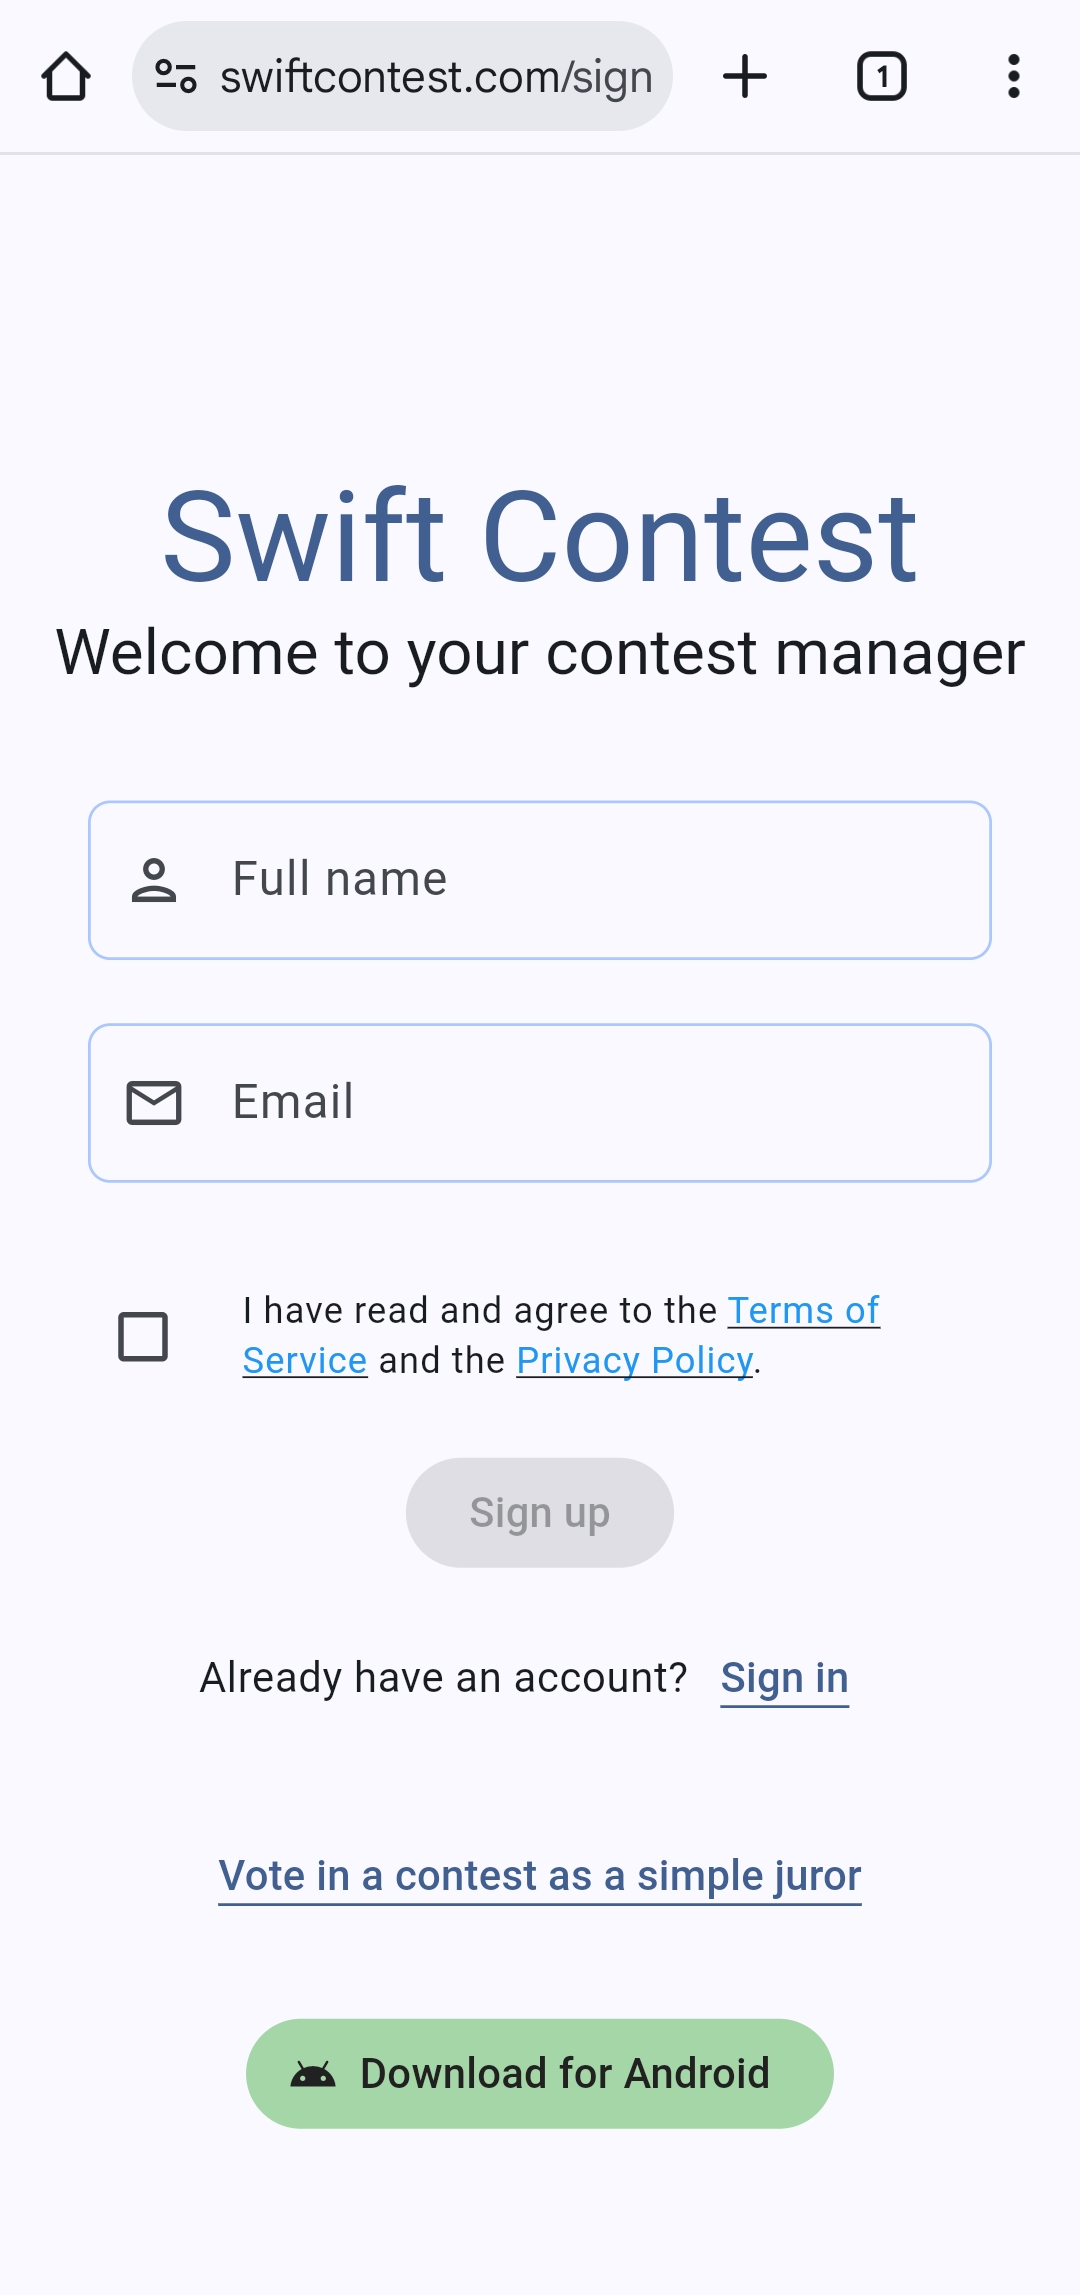
\includegraphics[width=0.4\textwidth]{images/web-sign-up}
    \caption{Pagina di accesso dell'applicazione web distribuita su Vercel.}
    \label{fig:web-sign-up}
\end{figure}

\section{Backend e Supabase}\label{sec:backend-e-supabase}
L'intera infrastruttura backend è gestita su Supabase.
Il processo di deployment del database è basato su migrazioni SQL, seguendo le pratiche di \textbf{Infrastructure as Code (IaC)}.
Ogni modifica allo schema del database, alle policy RLS o alle funzioni RPC è definita in un file \texttt{.sql} all'interno della cartella \texttt{supabase/migrations}.
La CLI di Supabase viene utilizzata per applicare queste migrazioni in modo sequenziale e versionato, garantendo che l'ambiente di produzione sia sempre allineato con la definizione del codice.
Le Edge Functions, scritte in TypeScript, vengono anch'esse deployate tramite la CLI\@.

% Tabella riassuntiva delle componenti Supabase
\begin{longtable}{p{0.2\textwidth} p{0.45\textwidth} p{0.3\textwidth}}
    \toprule
    \textbf{Componente} & \textbf{Utilizzo nel Progetto Swift Contest} & \textbf{Implementazione / Note Tecniche} \\
    \midrule
    \endfirsthead
    \toprule
    \textbf{Componente} & \textbf{Utilizzo nel Progetto Swift Contest} & \textbf{Implementazione / Note Tecniche} \\
    \midrule
    \endhead

    \textbf{Database} \newline (PostgreSQL) &
    Persistenza di tutti i dati applicativi: utenti, contest, partecipazioni, giurie, voti, ecc. È il "single source of truth" del sistema. &
    Schema e logica definiti tramite file di migrazione SQL nella cartella \texttt{supabase/migrations}. \\
    \midrule

    \textbf{Auth} &
    Gestione completa del ciclo di vita degli utenti: registrazione, login (email/password), autenticazione anonima per i giurati semplici e gestione delle sessioni tramite JWT. &
    Integrato tramite la libreria \texttt{supabase-flutter}.
    La tabella \texttt{auth.users} è estesa dalla tabella \texttt{public.profiles}. \\
    \midrule

    \textbf{Storage} &
    Archiviazione sicura di tutti i file binari caricati dagli utenti, come le immagini dei contest e i file dei \emph{Work}. &
    Nessun file è pubblico.
    L'accesso avviene esclusivamente tramite \emph{signed URL} temporanei generati lato server. \\
    \midrule

    \textbf{Edge Functions} &
    Esecuzione di logica server-side complessa, orchestrazione di operazioni multi-servizio (es.\ cancellazione utente da DB e Storage) e interazione con API esterne (Resend, Google Places).
    &
    Scritte in TypeScript (runtime Deno) e deployate dalla cartella \texttt{supabase/functions}. \\
    \midrule

    \textbf{Funzioni RPC} &
    Punto di ingresso primario per la logica di business confinata al database.
    Utilizzate per la maggior parte delle operazioni CRUD. &
    Scritte in PL/pgSQL e definite nei file di migrazione. \\
    \midrule

    \textbf{Realtime} &
    Propagazione di modifiche del database ai client sottoscritti in tempo reale.
    Utilizzato per le notifiche della \textbf{inbox} (tabella \texttt{messages}) e per aggiornare lo stato delle sessioni di voto.
    &
    L'autorizzazione alla sottoscrizione è gestita tramite policy RLS di tipo \texttt{SELECT}. \\

    \bottomrule \\
    \caption{Riepilogo delle componenti Supabase e del loro utilizzo nel progetto.}
    \label{tab:supabase_components}
\end{longtable}

\section{Dashboard amministrativa (Retool)}\label{sec:dashboard-amministrativa-(retool)}
Per le attività di amministrazione avanzata, come la moderazione degli utenti e la gestione dei contenuti, è stata creata una dashboard interna utilizzando \textbf{Retool}.
Questa interfaccia, non esposta agli utenti finali, comunica con il backend Supabase attraverso l'API sicura descritta nel capitolo precedente, utilizzando un utente di database dedicato per le letture ed Edge Functions protette da API-Key per le operazioni di scrittura.

\begin{figure}[H]
    \centering
    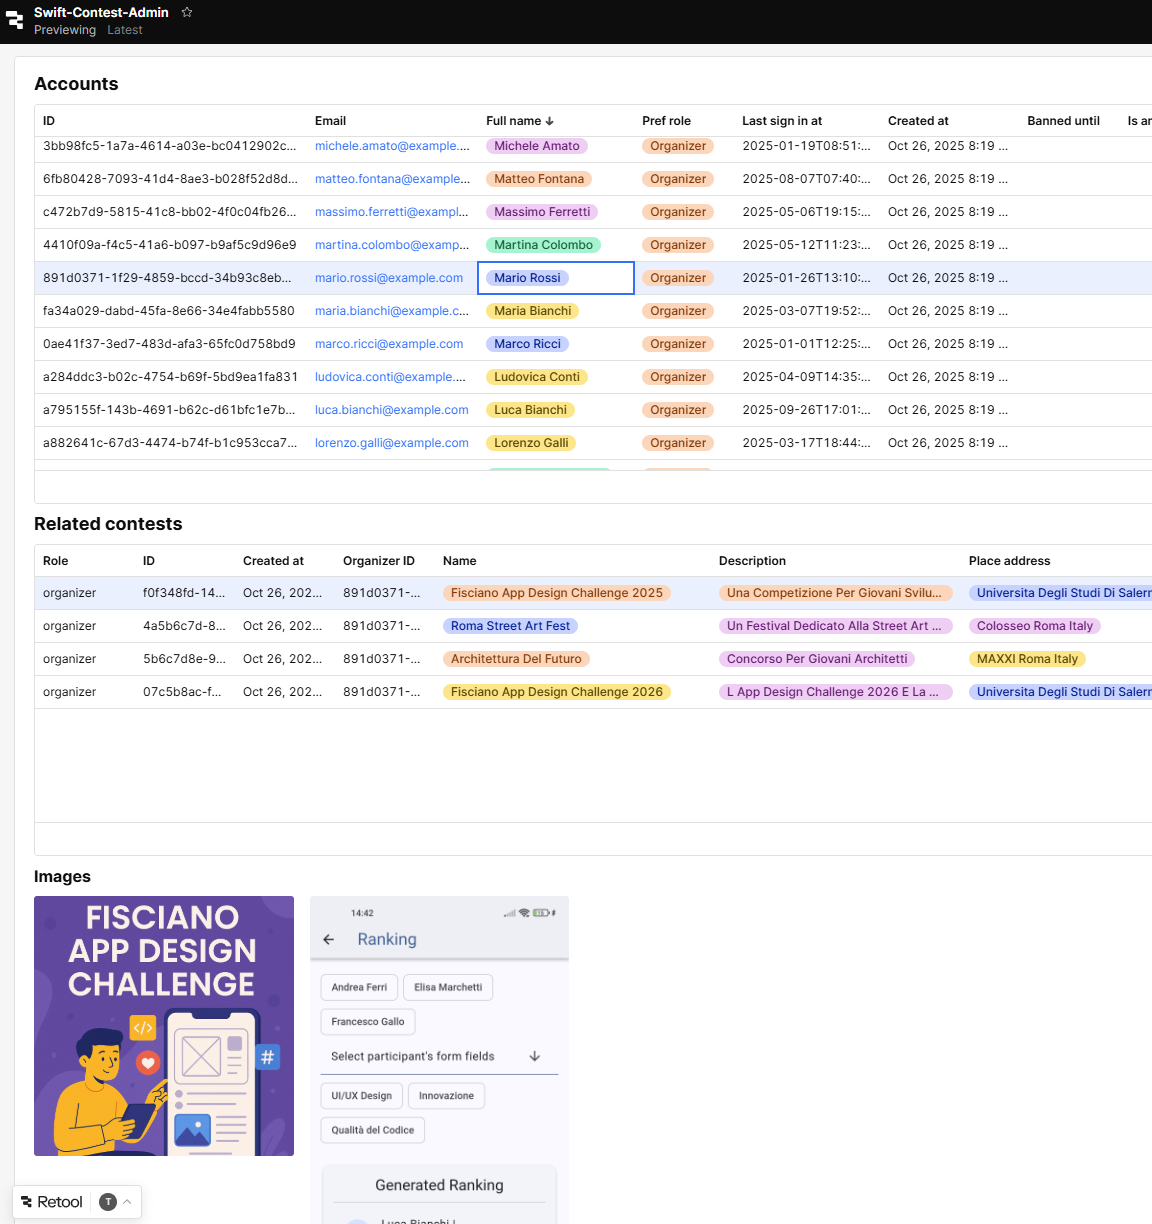
\includegraphics[width=0.8\textwidth]{images/retool-dashboard}
    \caption{La dashboard di amministrazione sviluppata in Retool.}
    \label{fig:retool-dashboard}
\end{figure}

\section{Prodotto finale: Interfaccia Utente e Flussi Operativi}\label{sec:prodotto-finale}
In questa sezione viene presentato il prodotto finale attraverso un'analisi visuale della sua interfaccia utente (UI).
Partendo dalle schermate di base, come l'autenticazione e le impostazioni, verranno poi illustrati i flussi operativi specifici per ciascuno degli attori del sistema: l'Organizzatore, il Partecipante e il Giurato.

\subsection{Accesso e Autenticazione}\label{subsec:accesso-e-autenticazione}
L'accesso all'applicazione inizia con una \textbf{Splash Screen} che gestisce l'inizializzazione dei servizi principali.
Successivamente, l'utente viene indirizzato al flusso di autenticazione, che comprende le pagine di \textbf{Sign In} (per l'accesso), \textbf{Sign Up} (per la registrazione di un nuovo account) e le relative schermate per la verifica dell'email.
L'interfaccia è stata progettata per essere pulita, minimale e coerente con le linee guida del Material Design 3.

% --- Esempio con immagini affiancate (CONSIGLIATO) ---
\begin{figure}[H]
    \centering
    \begin{minipage}{0.32\textwidth}
        \centering
        
\includegraphics[width=\linewidth]{images/splash}
        \subcaption{Splash Screen}
        \label{fig:splash}
    \end{minipage}\hfill %
    \begin{minipage}{0.32\textwidth}
        \centering
        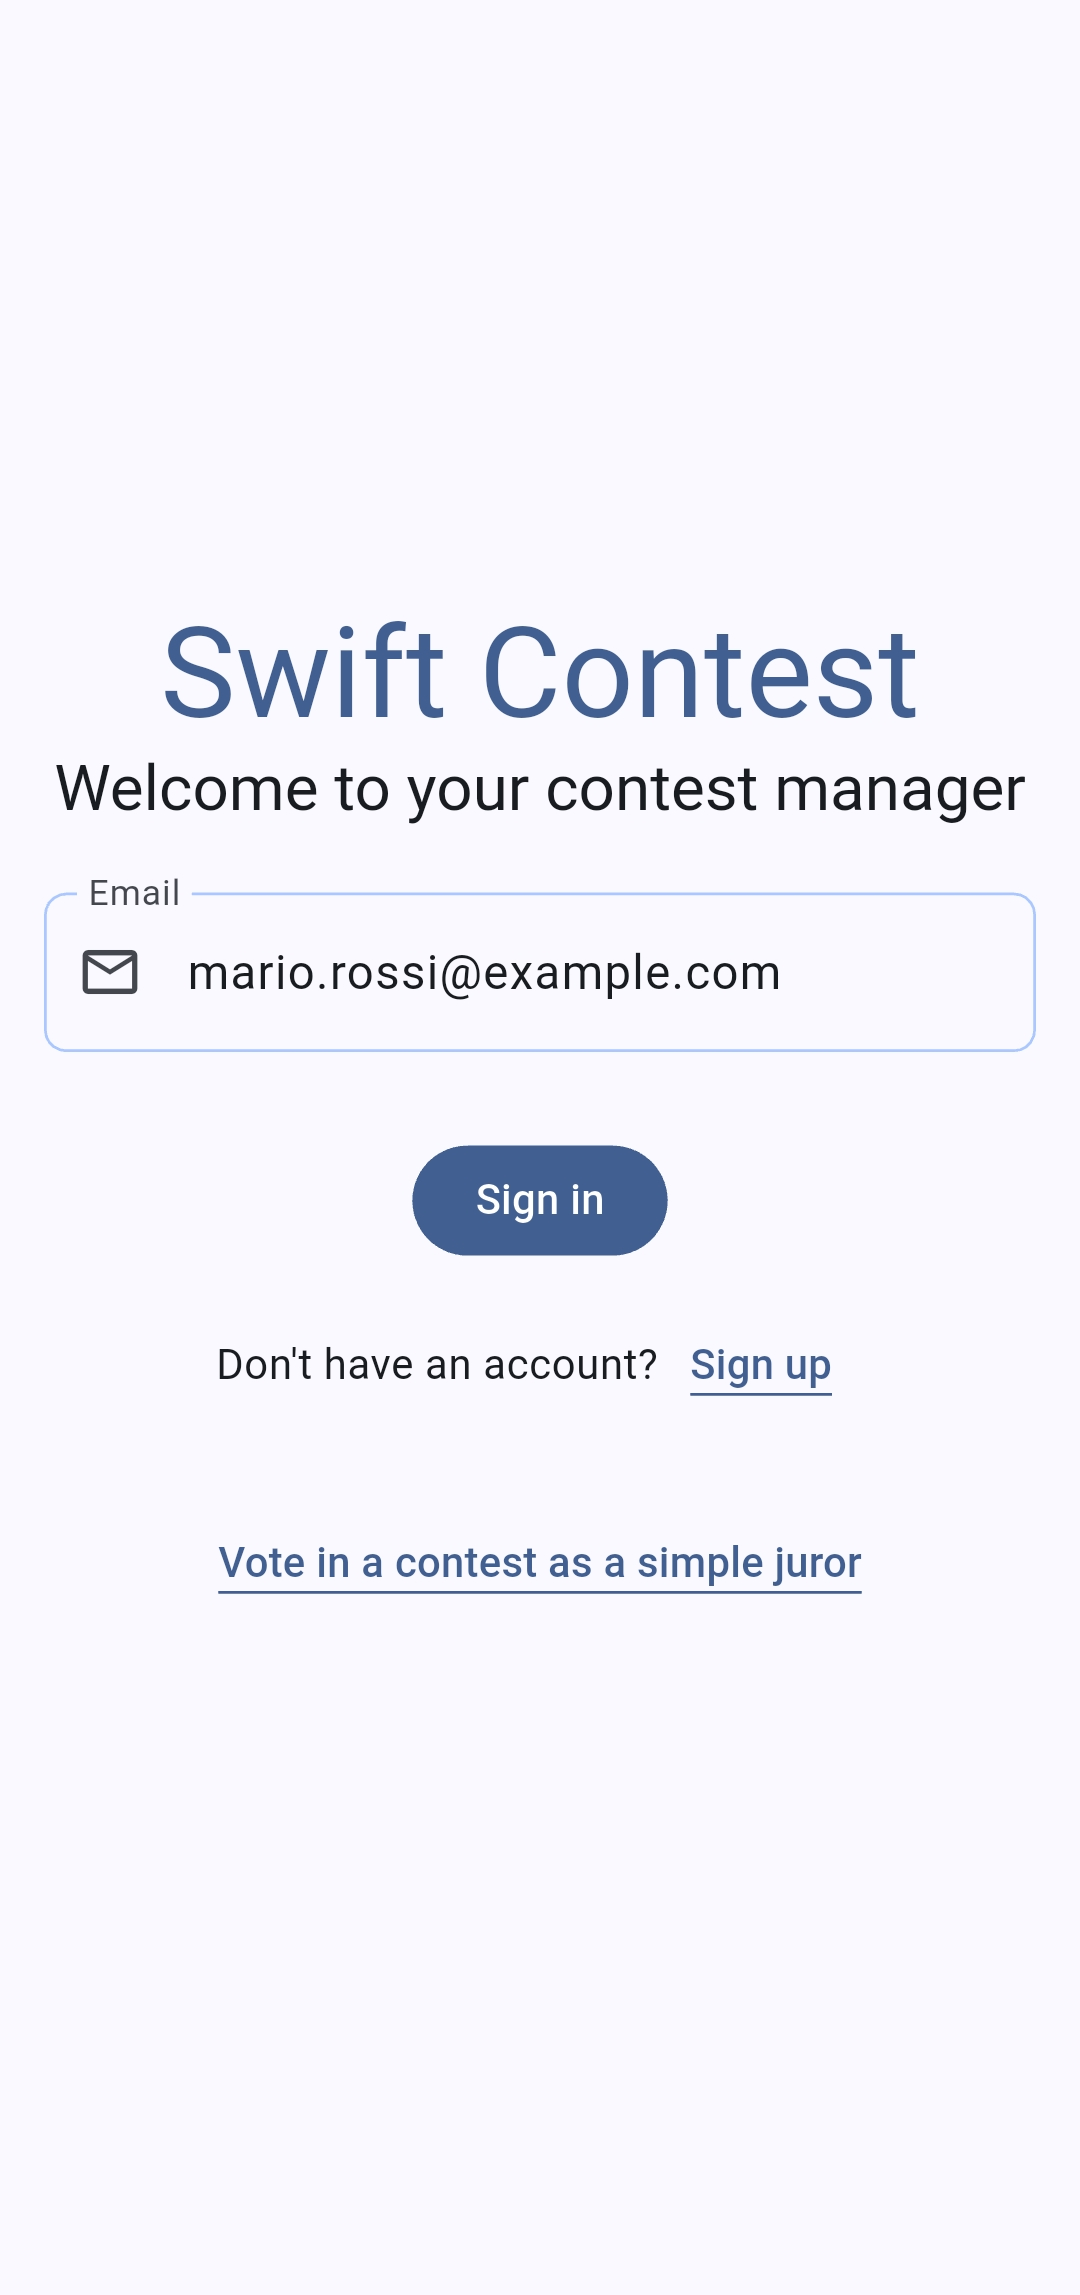
\includegraphics[width=\linewidth]{images/sign-in}
        \subcaption{Pagina di Sign In}
        \label{fig:signin}
    \end{minipage}\hfill %
    \begin{minipage}{0.32\textwidth}
        \centering
        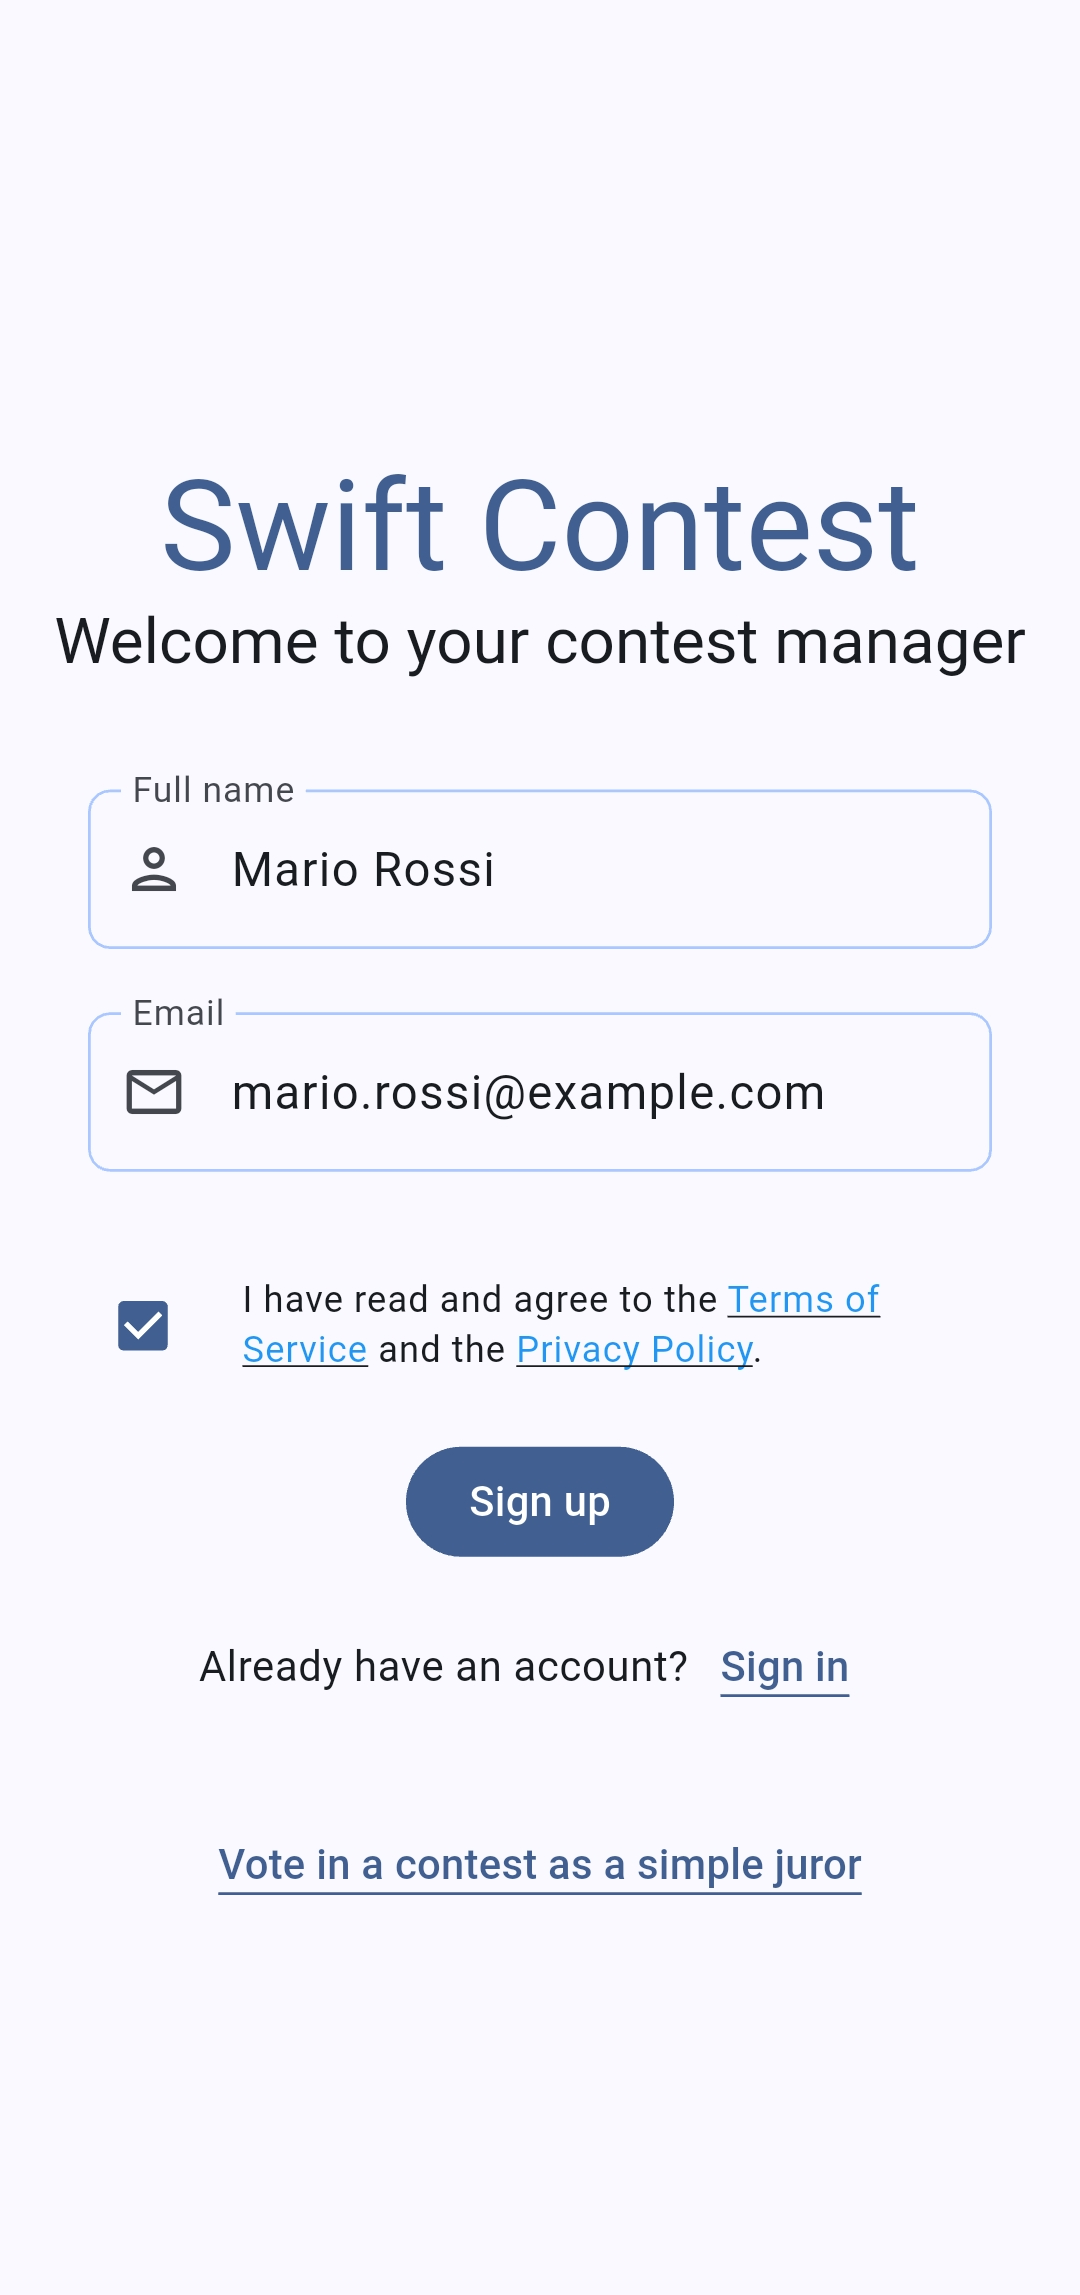
\includegraphics[width=\linewidth]{images/sign-up}
        \subcaption{Pagina di Sign Up}
        \label{fig:signup}
    \end{minipage}
    \caption{Le schermate del flusso di autenticazione dell'applicazione.}
    \label{fig:auth-flow}
\end{figure}

\subsection{Gestione delle Impostazioni}\label{subsec:gestione-impostazioni}
Una volta autenticato, ogni utente ha accesso a una sezione dedicata alle impostazioni.
Da qui, l'utente può navigare alla pagina \textbf{Impostazioni Account}, dove può modificare i dati del proprio profilo (come il nome completo) o procedere con l'eliminazione sicura e autonoma del proprio account.

% --- Esempio con due immagini affiancate ---
\begin{figure}[H]
    \centering
    \begin{minipage}{0.48\textwidth}
        \centering
        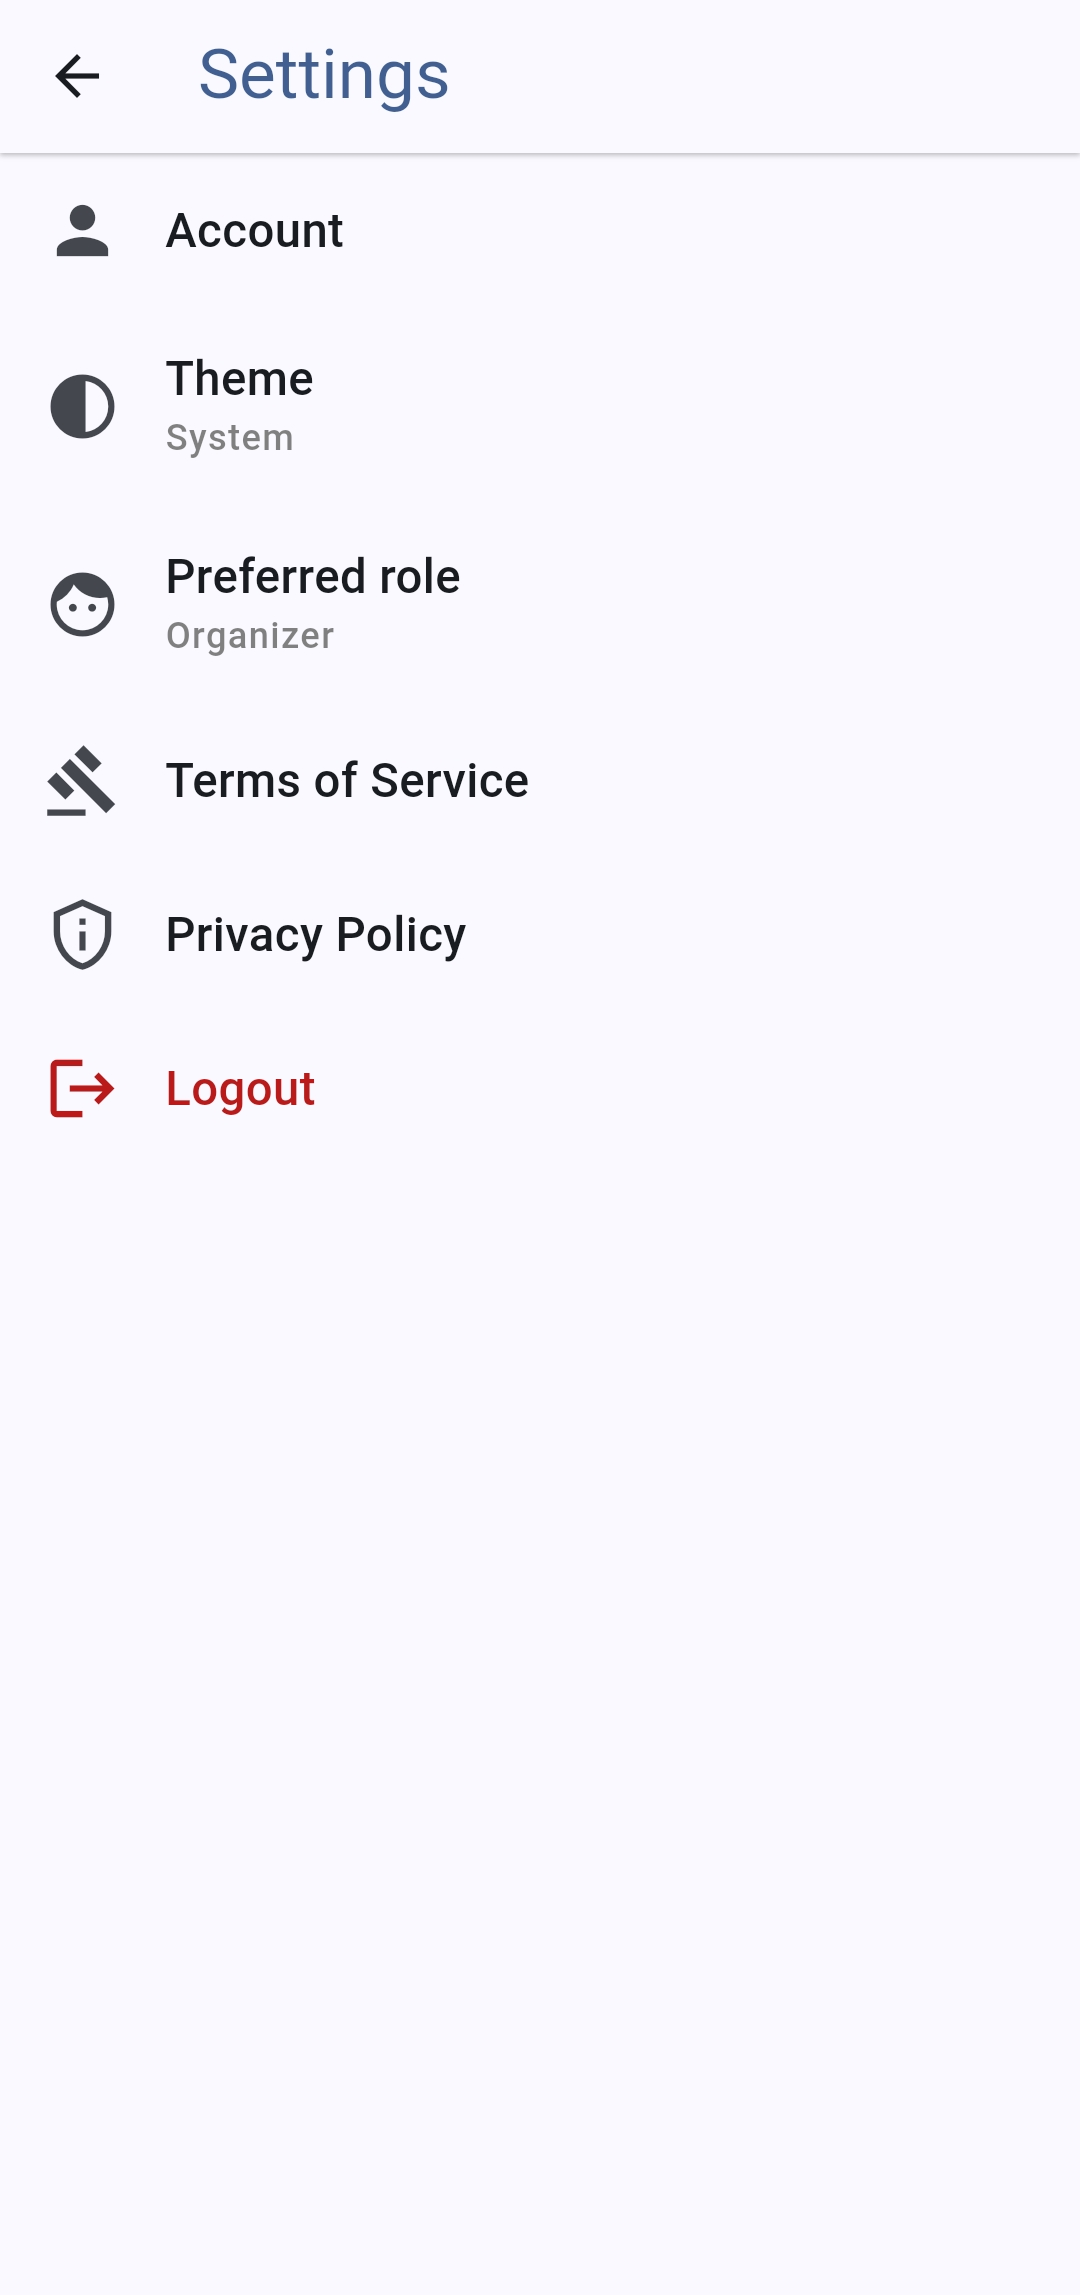
\includegraphics[width=\linewidth]{images/settings}
        \subcaption{Pagina delle Impostazioni Generali}
        \label{fig:settings}
    \end{minipage}\hfill %
    \begin{minipage}{0.48\textwidth}
        \centering
        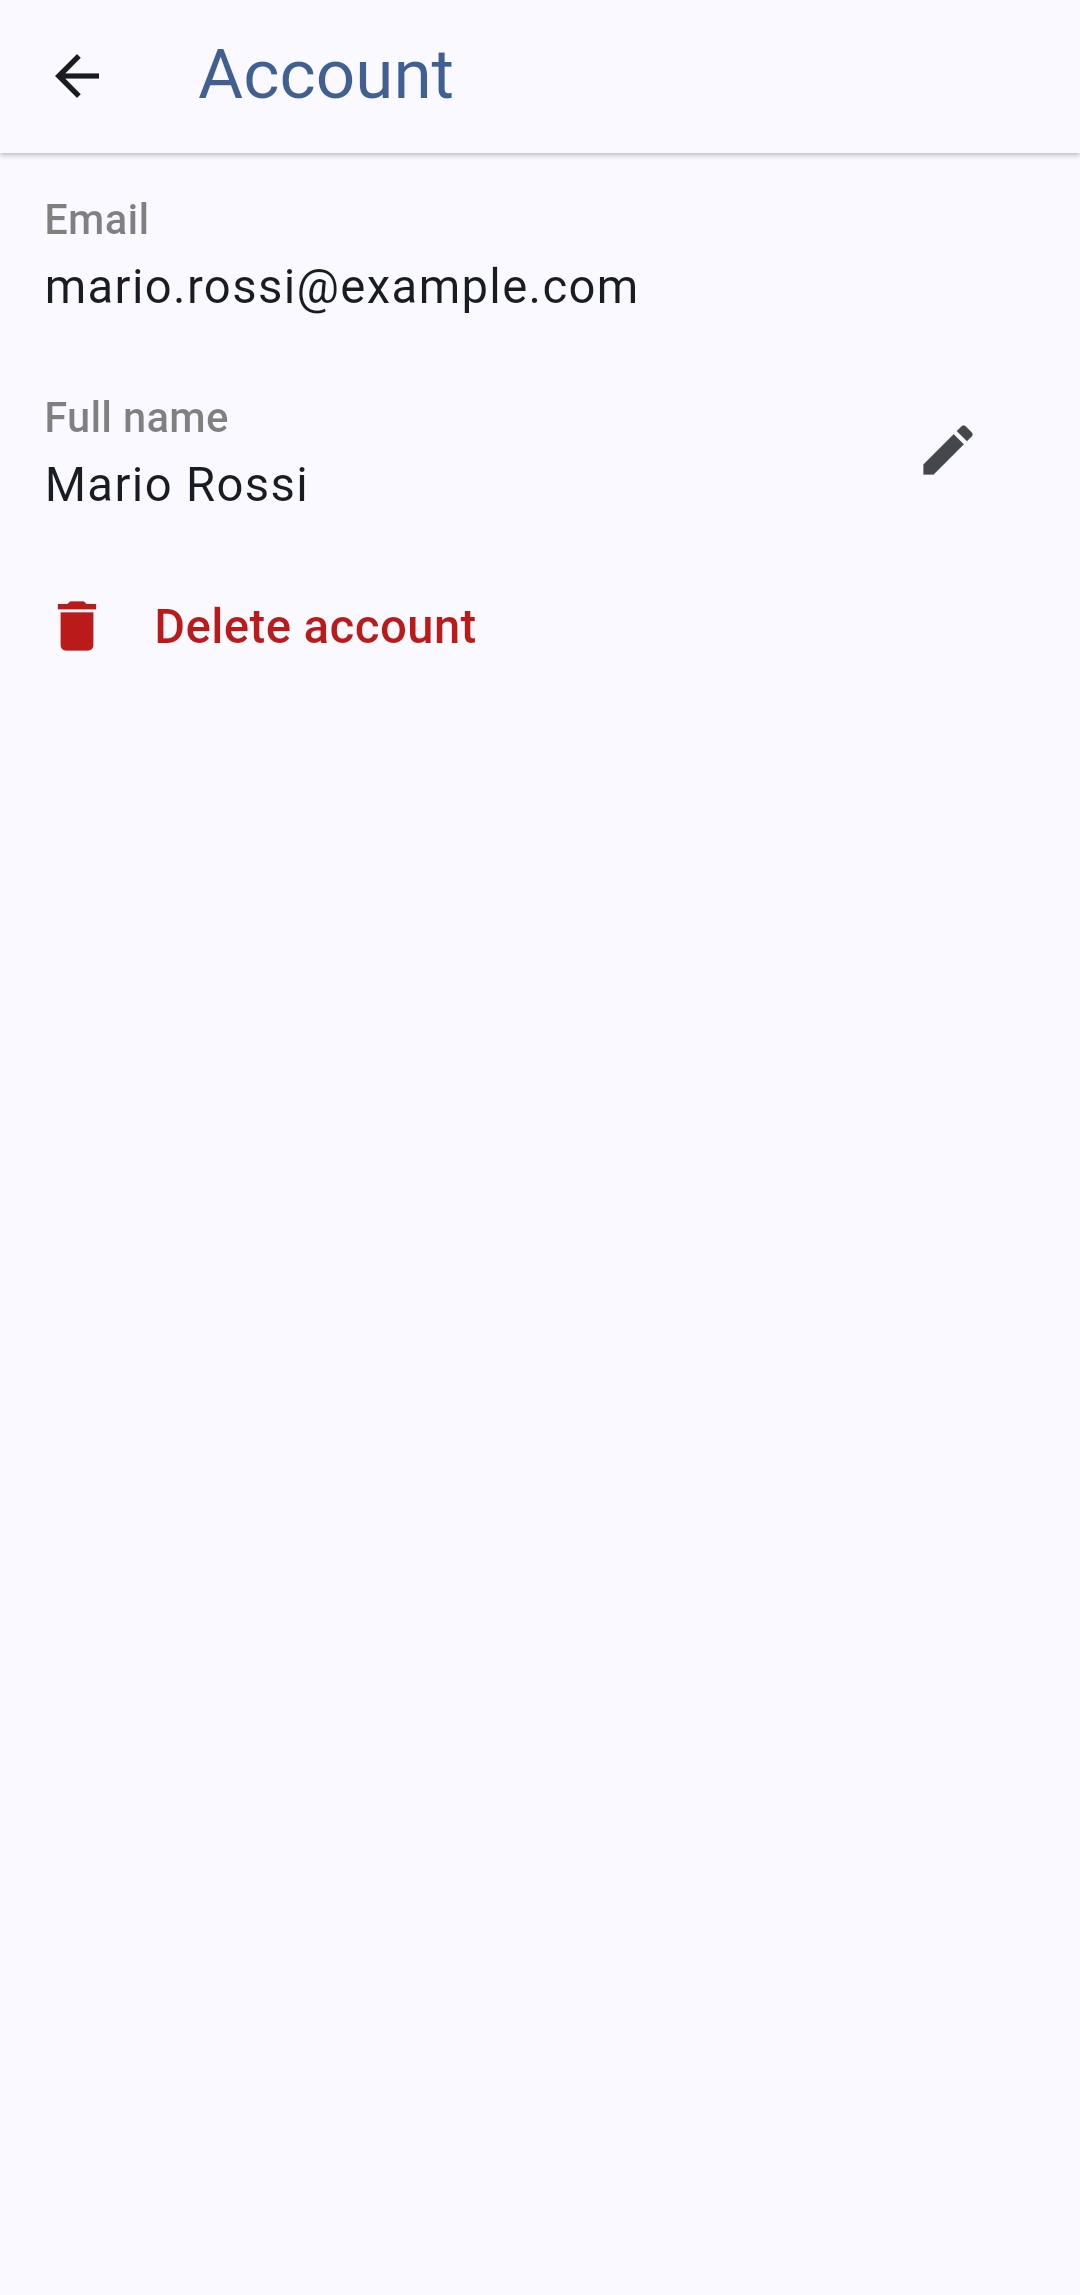
\includegraphics[width=\linewidth]{images/account-settings}
        \subcaption{Pagina Impostazioni Account}
        \label{fig:account_settings}
    \end{minipage}
    \caption{Le schermate per la gestione delle impostazioni dell'app e dell'account utente.}
    \label{fig:settings-flow}
\end{figure}

\subsection{Flusso dell'Organizzatore}\label{subsec:flusso-organizzatore}
L'organizzatore è l'attore con il set di funzionalità più ricco, responsabile dell'intero ciclo di vita del contest.
Il suo percorso inizia dalla \textbf{Home Page}, che funge da dashboard principale, mostrando l'elenco dei contest da lui creati e fornendo l'accesso a tutte le funzionalità principali.

% --- FIGURA: Home Page Organizzatore ---
\begin{figure}[H]
    \centering
    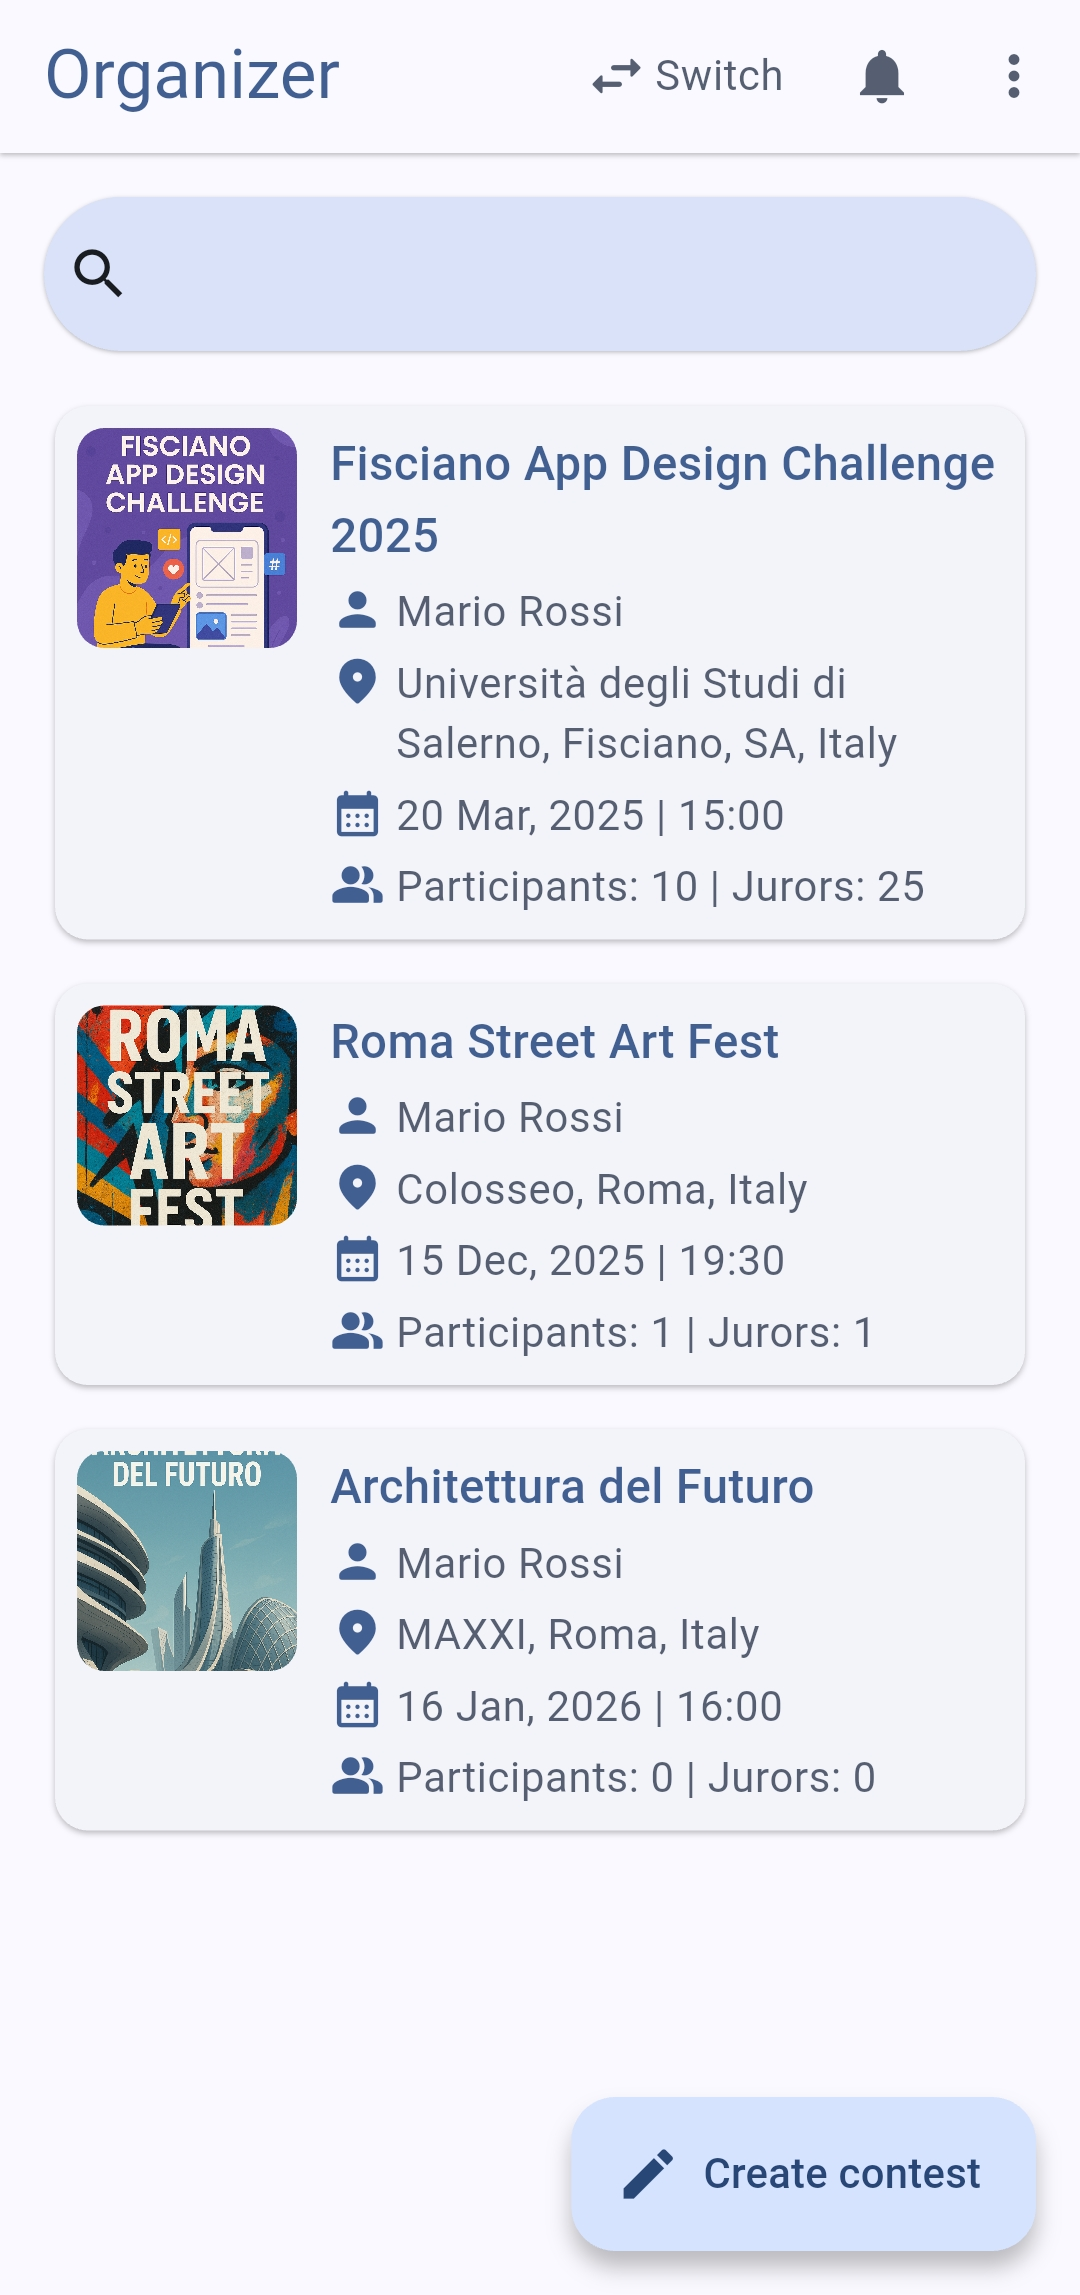
\includegraphics[width=0.4\textwidth]{images/organizer-home}
    \caption{La Home Page dell'Organizzatore, con l'elenco dei contest gestiti.}
    \label{fig:organizer_home}
\end{figure}

\paragraph{Primo Flusso: Creazione di un Nuovo Contest}
Dalla home page, l'organizzatore può avviare la creazione di un nuovo contest.
Viene guidato attraverso un \textbf{form multi-step} che semplifica l'inserimento di tutte le informazioni necessarie, suddivise in tre passaggi logici:
\begin{enumerate}
    \item \textbf{Informazioni di Base}: nome, descrizione e immagini rappresentative.
    \item \textbf{Date e Scadenze}: data dell'evento e periodo per la sottomissione dei lavori.
    \item \textbf{Luogo}: selezione del luogo tramite un'interfaccia integrata con l'API di Google Places.
\end{enumerate}
Una volta completato, il nuovo contest appare nella sua dashboard, pronto per essere configurato.

% --- FIGURE: Creazione Contest (3 immagini affiancate) ---
\begin{figure}[H]
    \centering
    \begin{minipage}{0.32\textwidth}
        \centering
        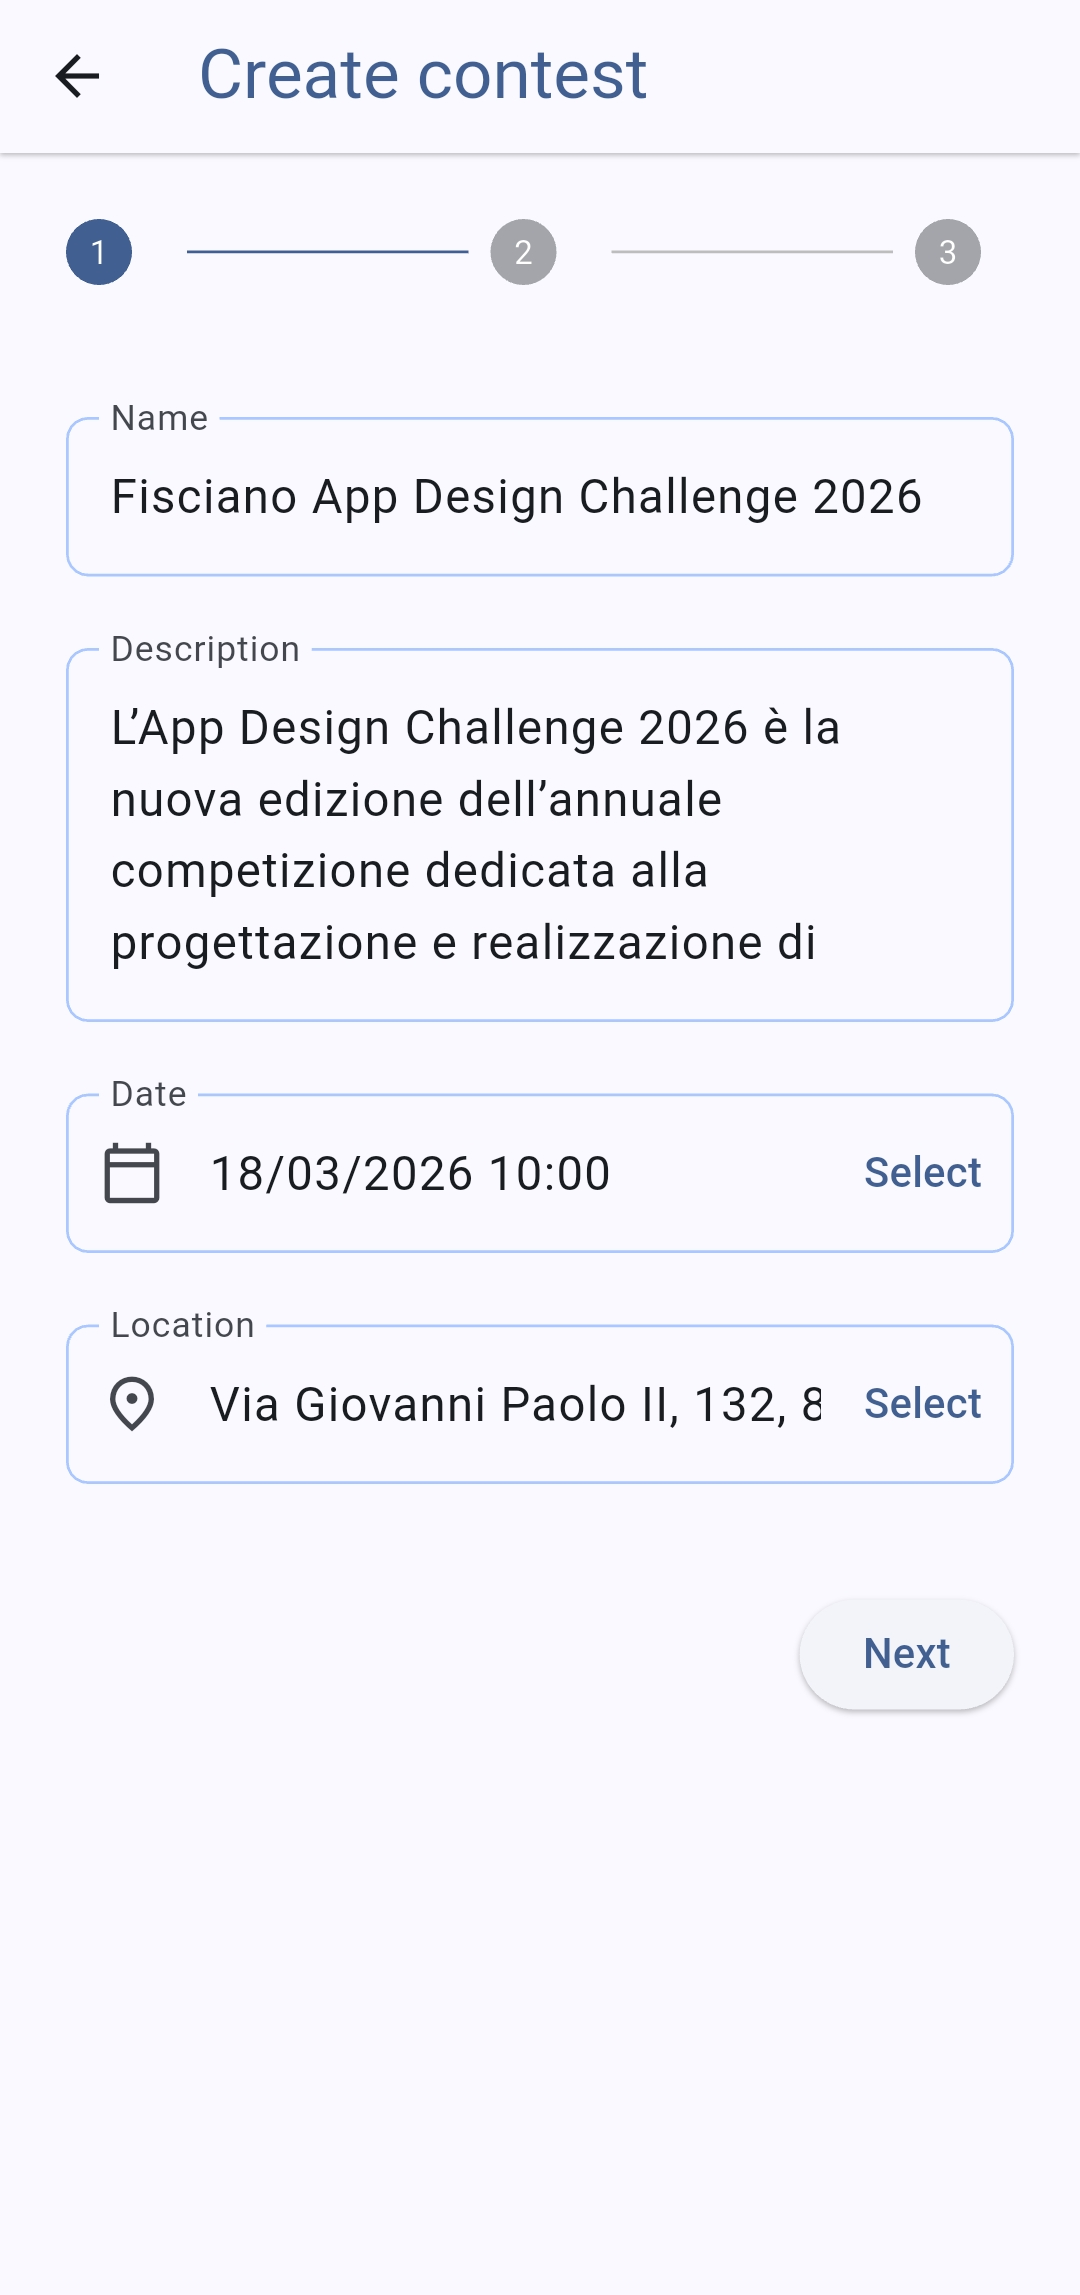
\includegraphics[width=\linewidth]{images/organizer-create-contest-step1}
        \subcaption{Passo 1: Info Base}
        \label{fig:create_contest_1}
    \end{minipage}\hfill
    \begin{minipage}{0.32\textwidth}
        \centering
        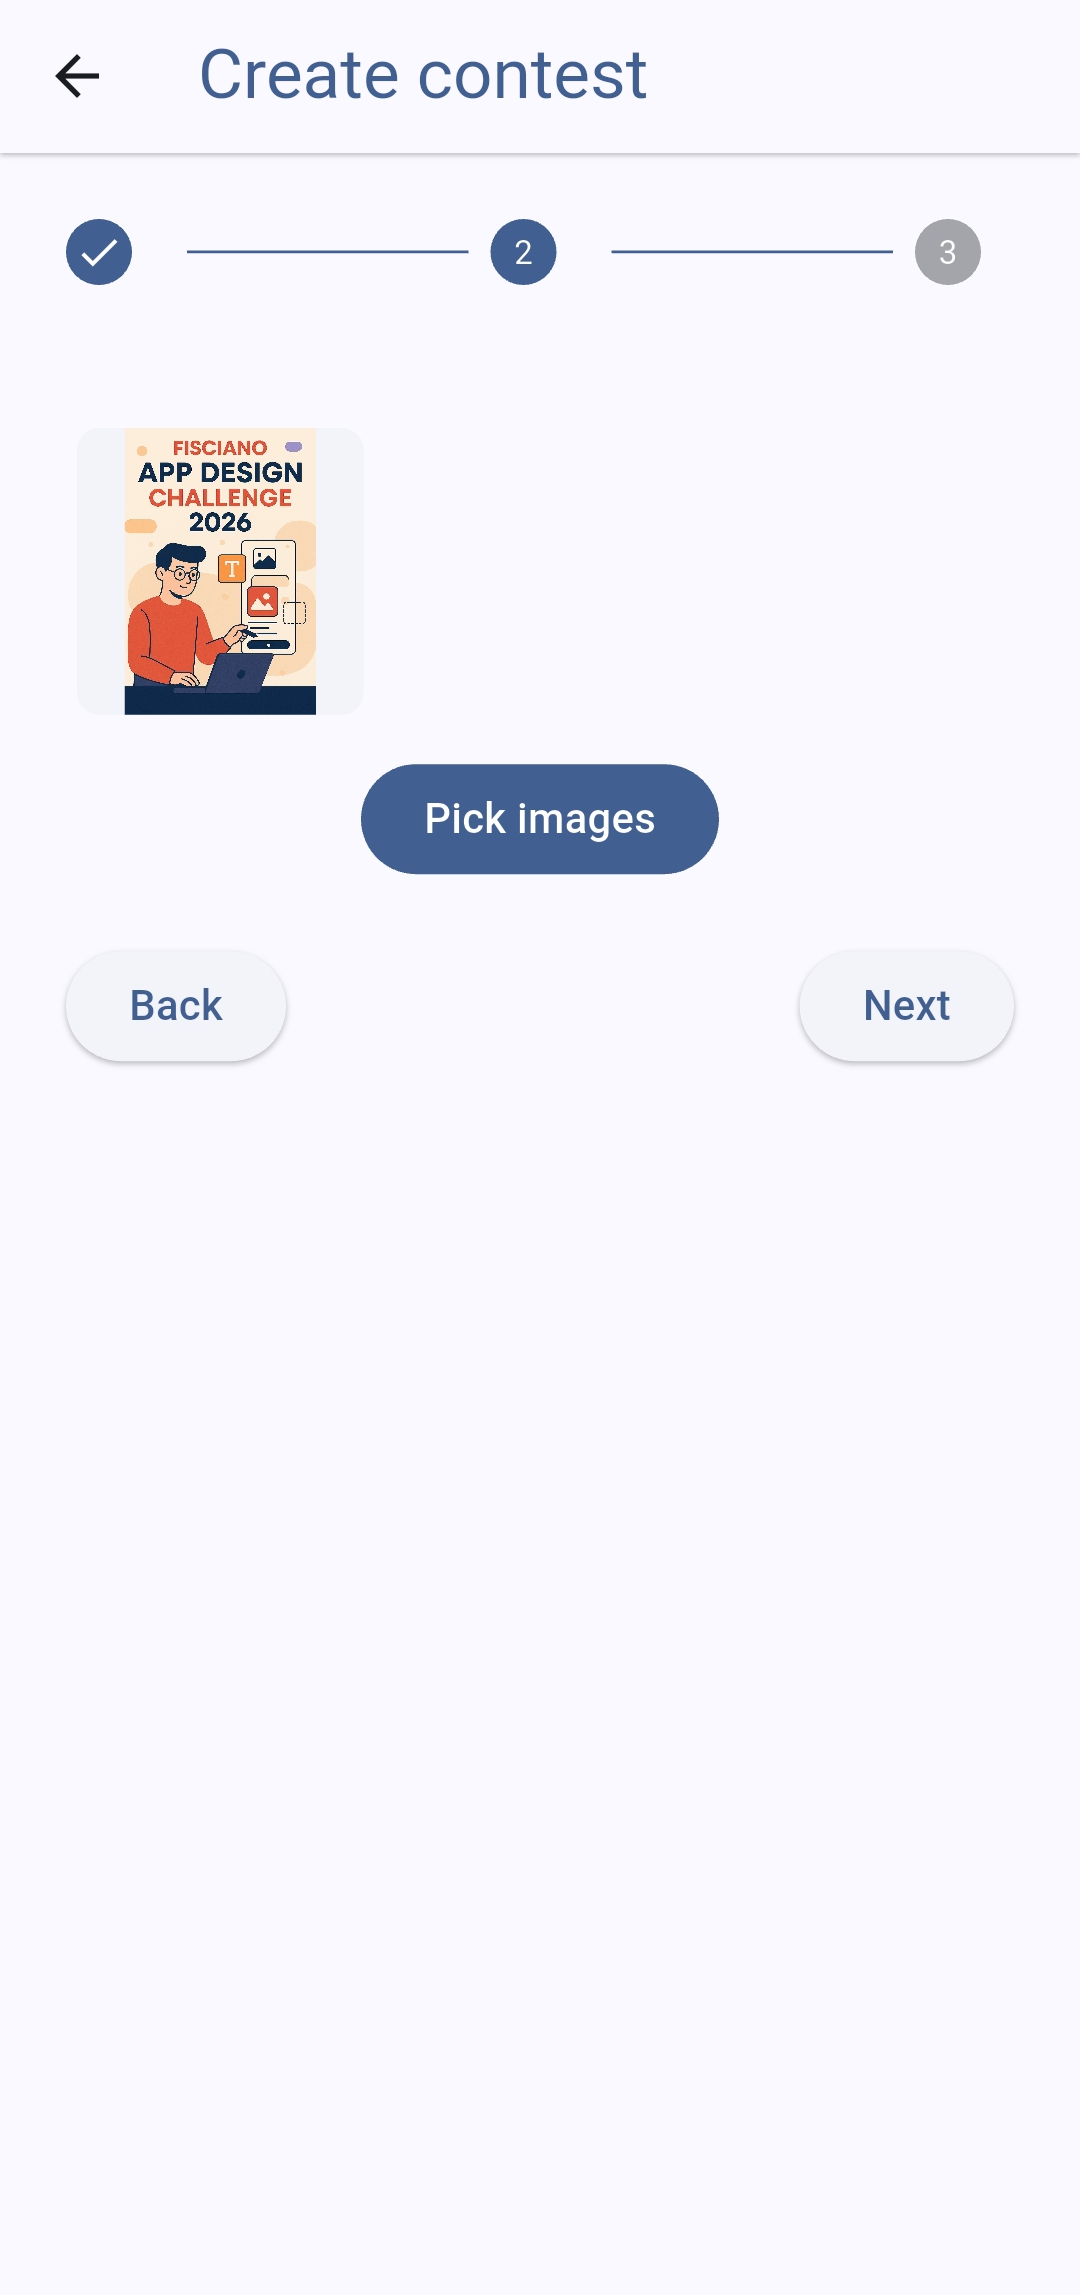
\includegraphics[width=\linewidth]{images/organizer-create-contest-step2}
        \subcaption{Passo 2: Date}
        \label{fig:create_contest_2}
    \end{minipage}\hfill
    \begin{minipage}{0.32\textwidth}
        \centering
        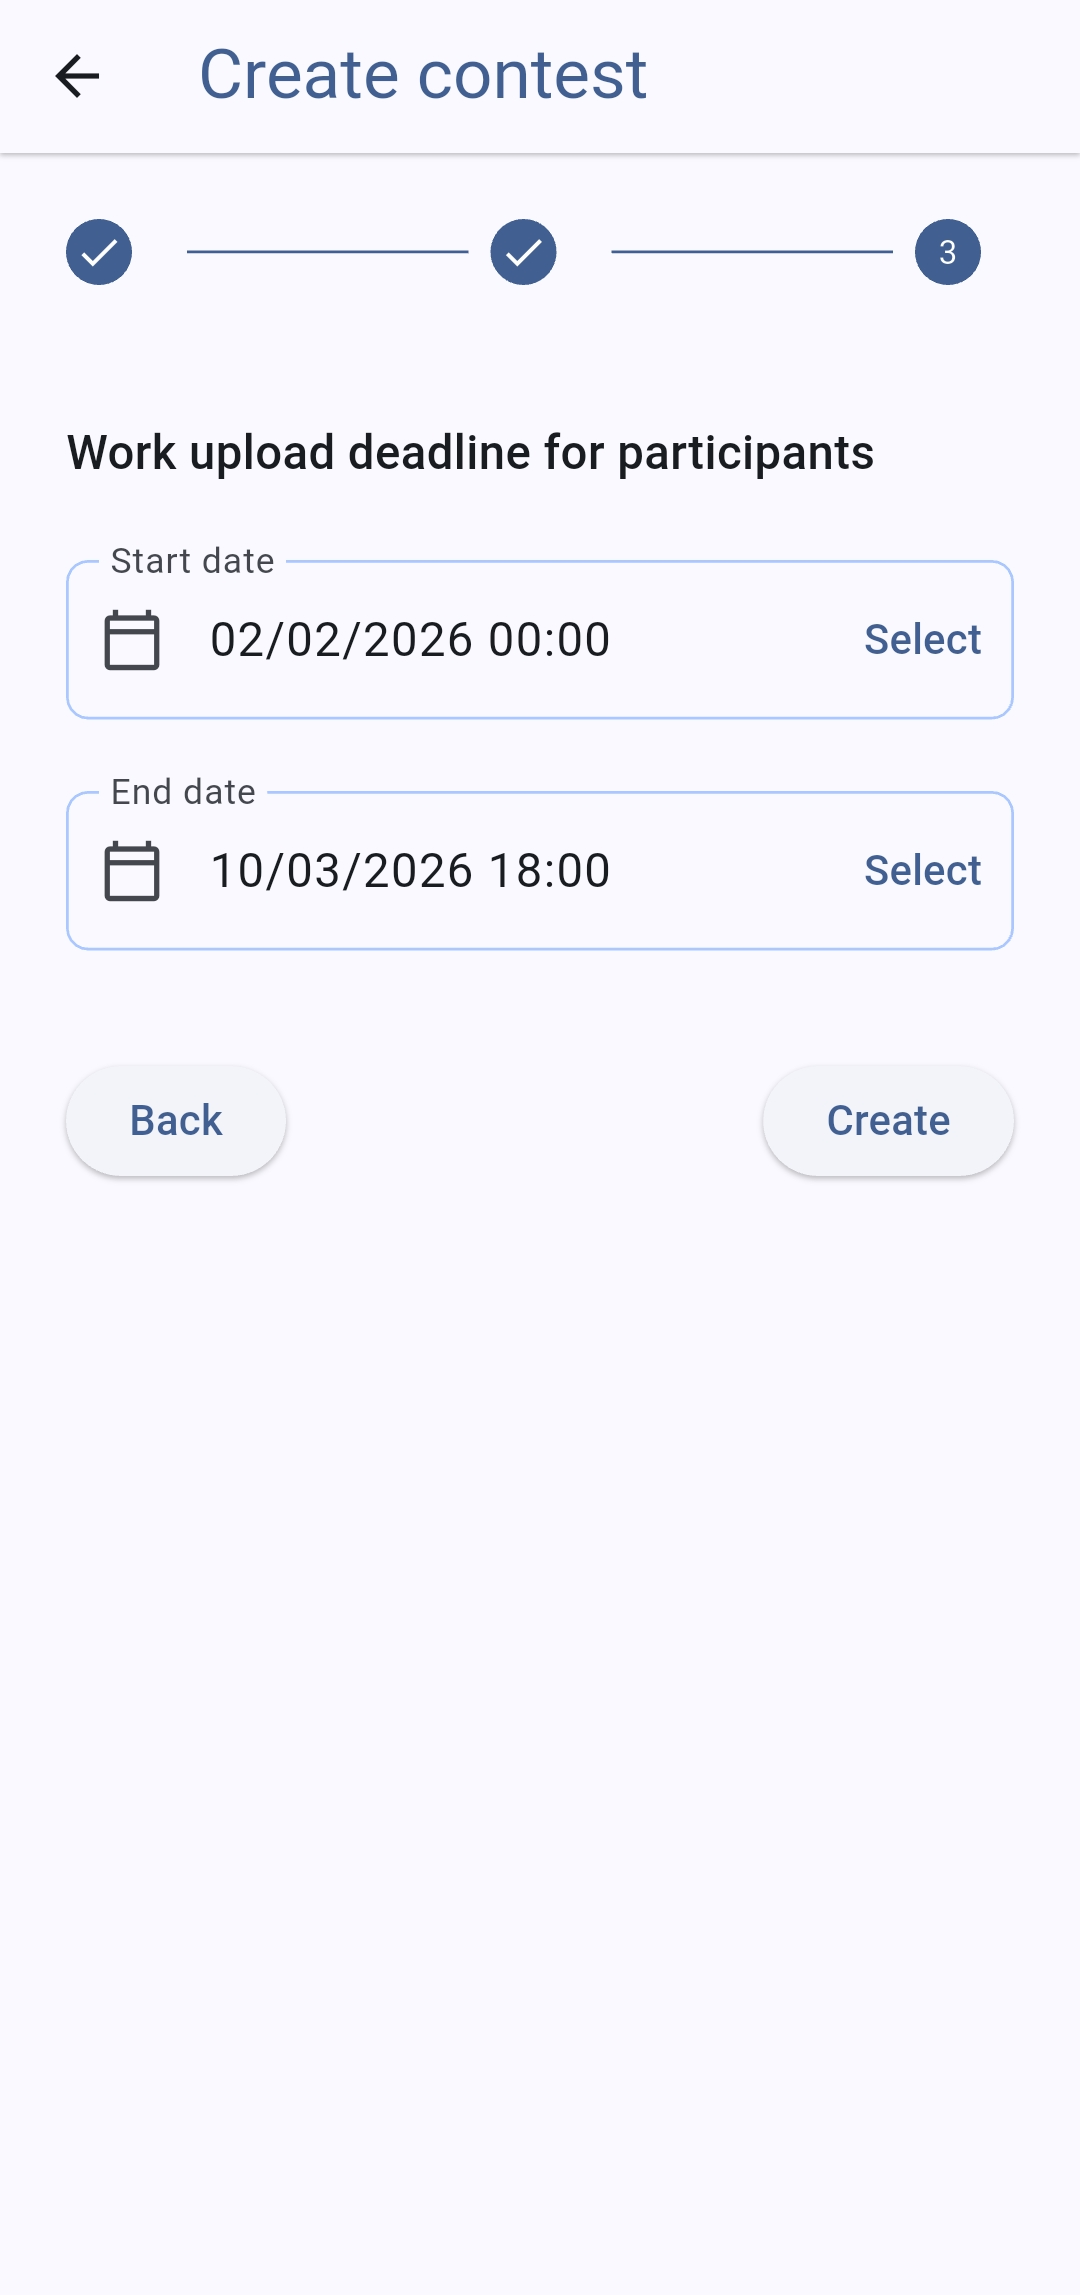
\includegraphics[width=\linewidth]{images/organizer-create-contest-step3}
        \subcaption{Passo 3: Luogo}
        \label{fig:create_contest_3}
    \end{minipage}
    \caption{Le tre schermate del form guidato per la creazione di un nuovo contest.}
    \label{fig:create_contest_flow}
\end{figure}

\paragraph{Secondo Flusso: Configurazione dei Dettagli del Contest}
Selezionando un contest dalla home page, l'organizzatore accede al pannello di gestione, organizzato in tab.
Da qui può configurare ogni aspetto del contest:
\begin{itemize}
    \item La tab \textbf{Details} permette di modificare le informazioni generali.
    \item La tab \textbf{Participants} mostra l'elenco dei partecipanti iscritti e permette di inviarne di nuovi.
    \item La tab \textbf{Juries} consente di creare e gestire le giurie e di configurare il \textbf{Voting Form} associato a ciascuna, definendone i campi.
    \item La tab \textbf{Works} mostra l'elenco dei lavori sottomessi dai partecipanti.
\end{itemize}

% --- FIGURE: Dettagli Contest (4 immagini, 2 per riga) ---
\begin{figure}[H]
    \centering
    \begin{minipage}{0.48\textwidth}
        \centering
        
\includegraphics[width=\linewidth]{images/organizer-contest-details}
        \subcaption{Tab Details}
        \label{fig:contest_details}
    \end{minipage}\hfill
    \begin{minipage}{0.48\textwidth}
        \centering
        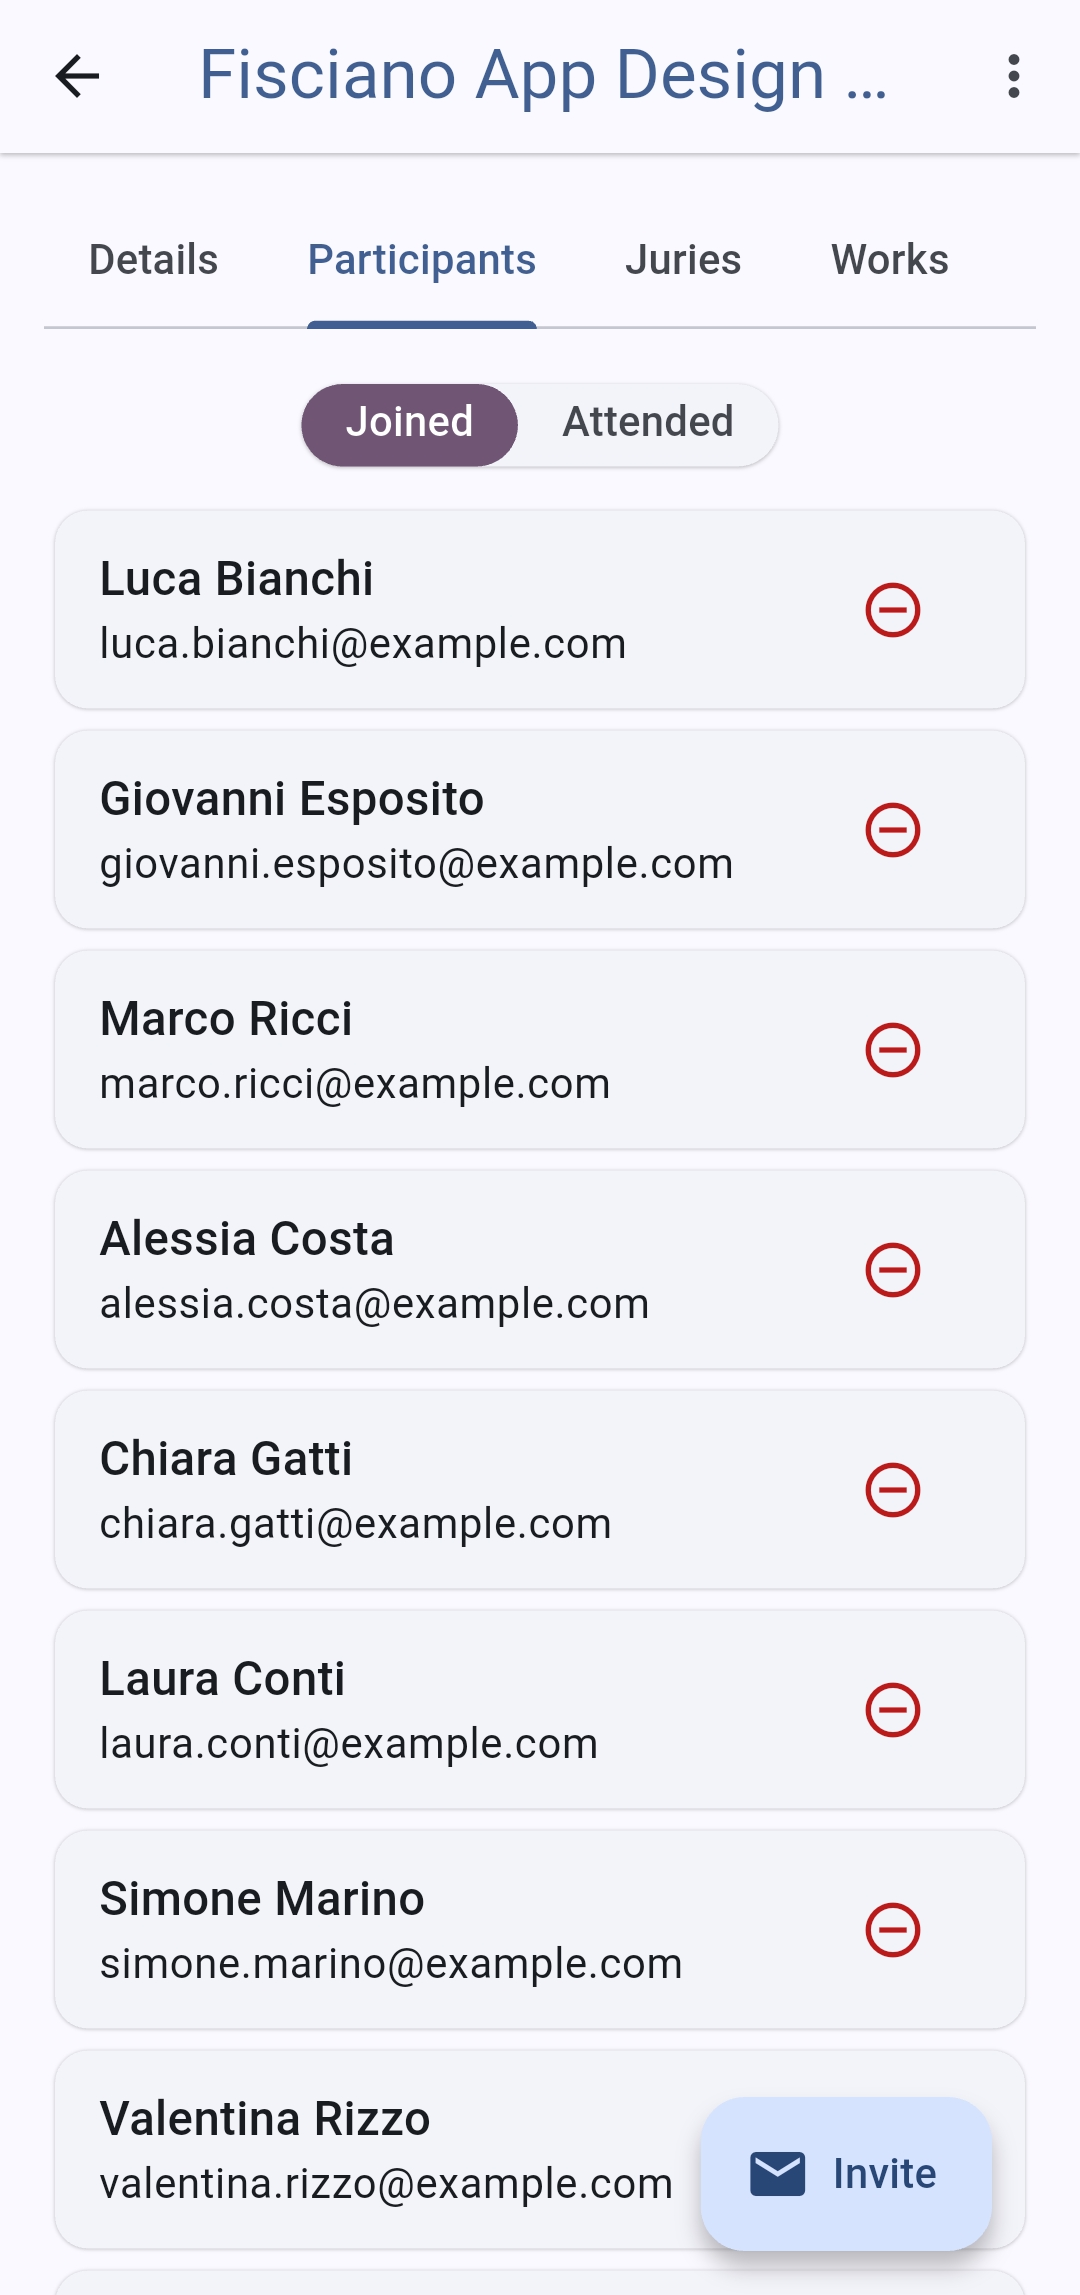
\includegraphics[width=\linewidth]{images/organizer-contest-participants}
        \subcaption{Tab Participants}
        \label{fig:contest_participants}
    \end{minipage}

    \vspace{1em} % Aggiunge spazio verticale tra le righe di immagini

    \begin{minipage}{0.48\textwidth}
        \centering
        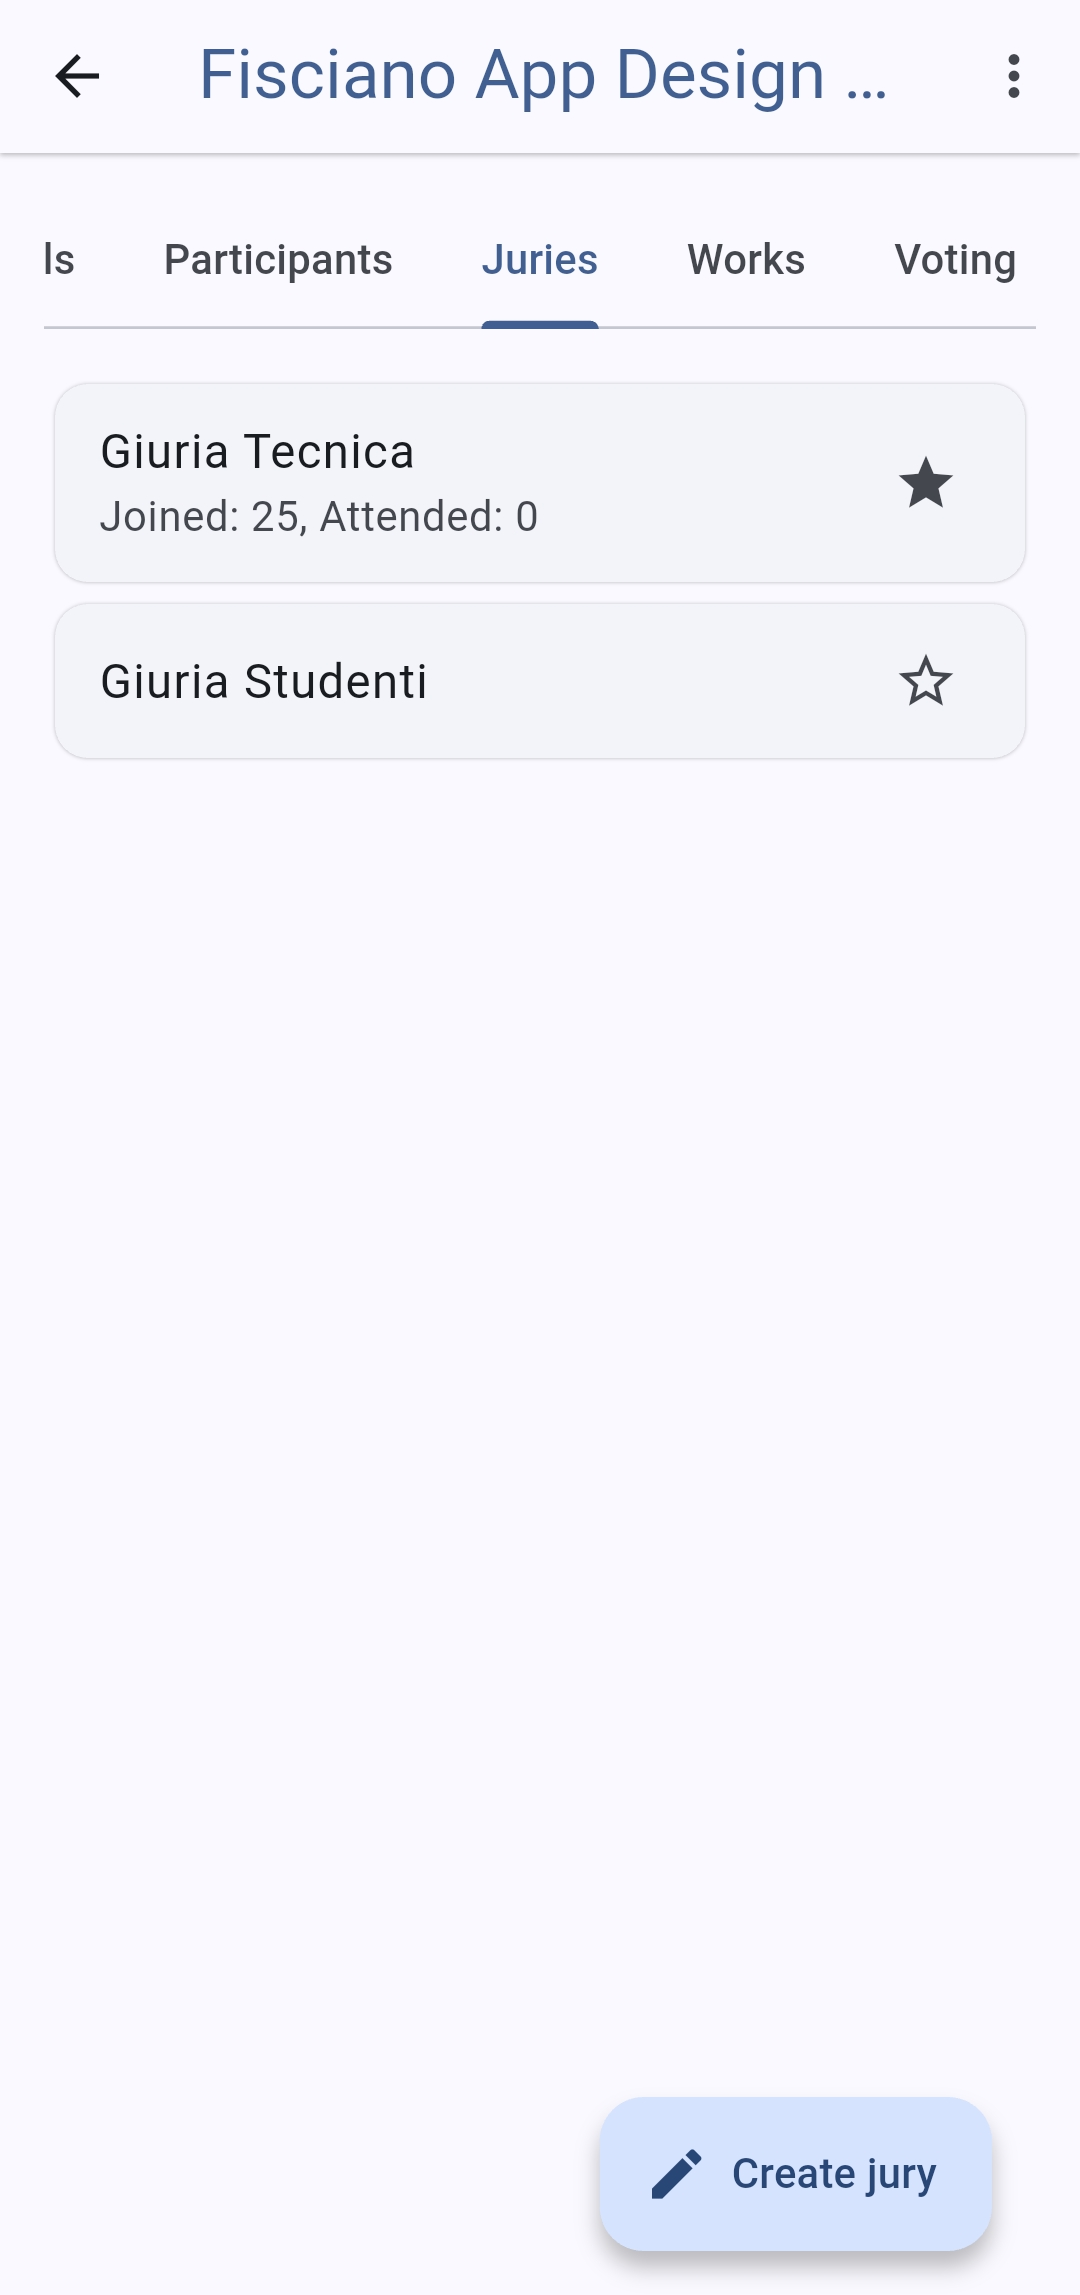
\includegraphics[width=\linewidth]{images/organizer-contest-juries}
        \subcaption{Tab Juries}
        \label{fig:contest_juries}
    \end{minipage}\hfill
    \begin{minipage}{0.48\textwidth}
        \centering
        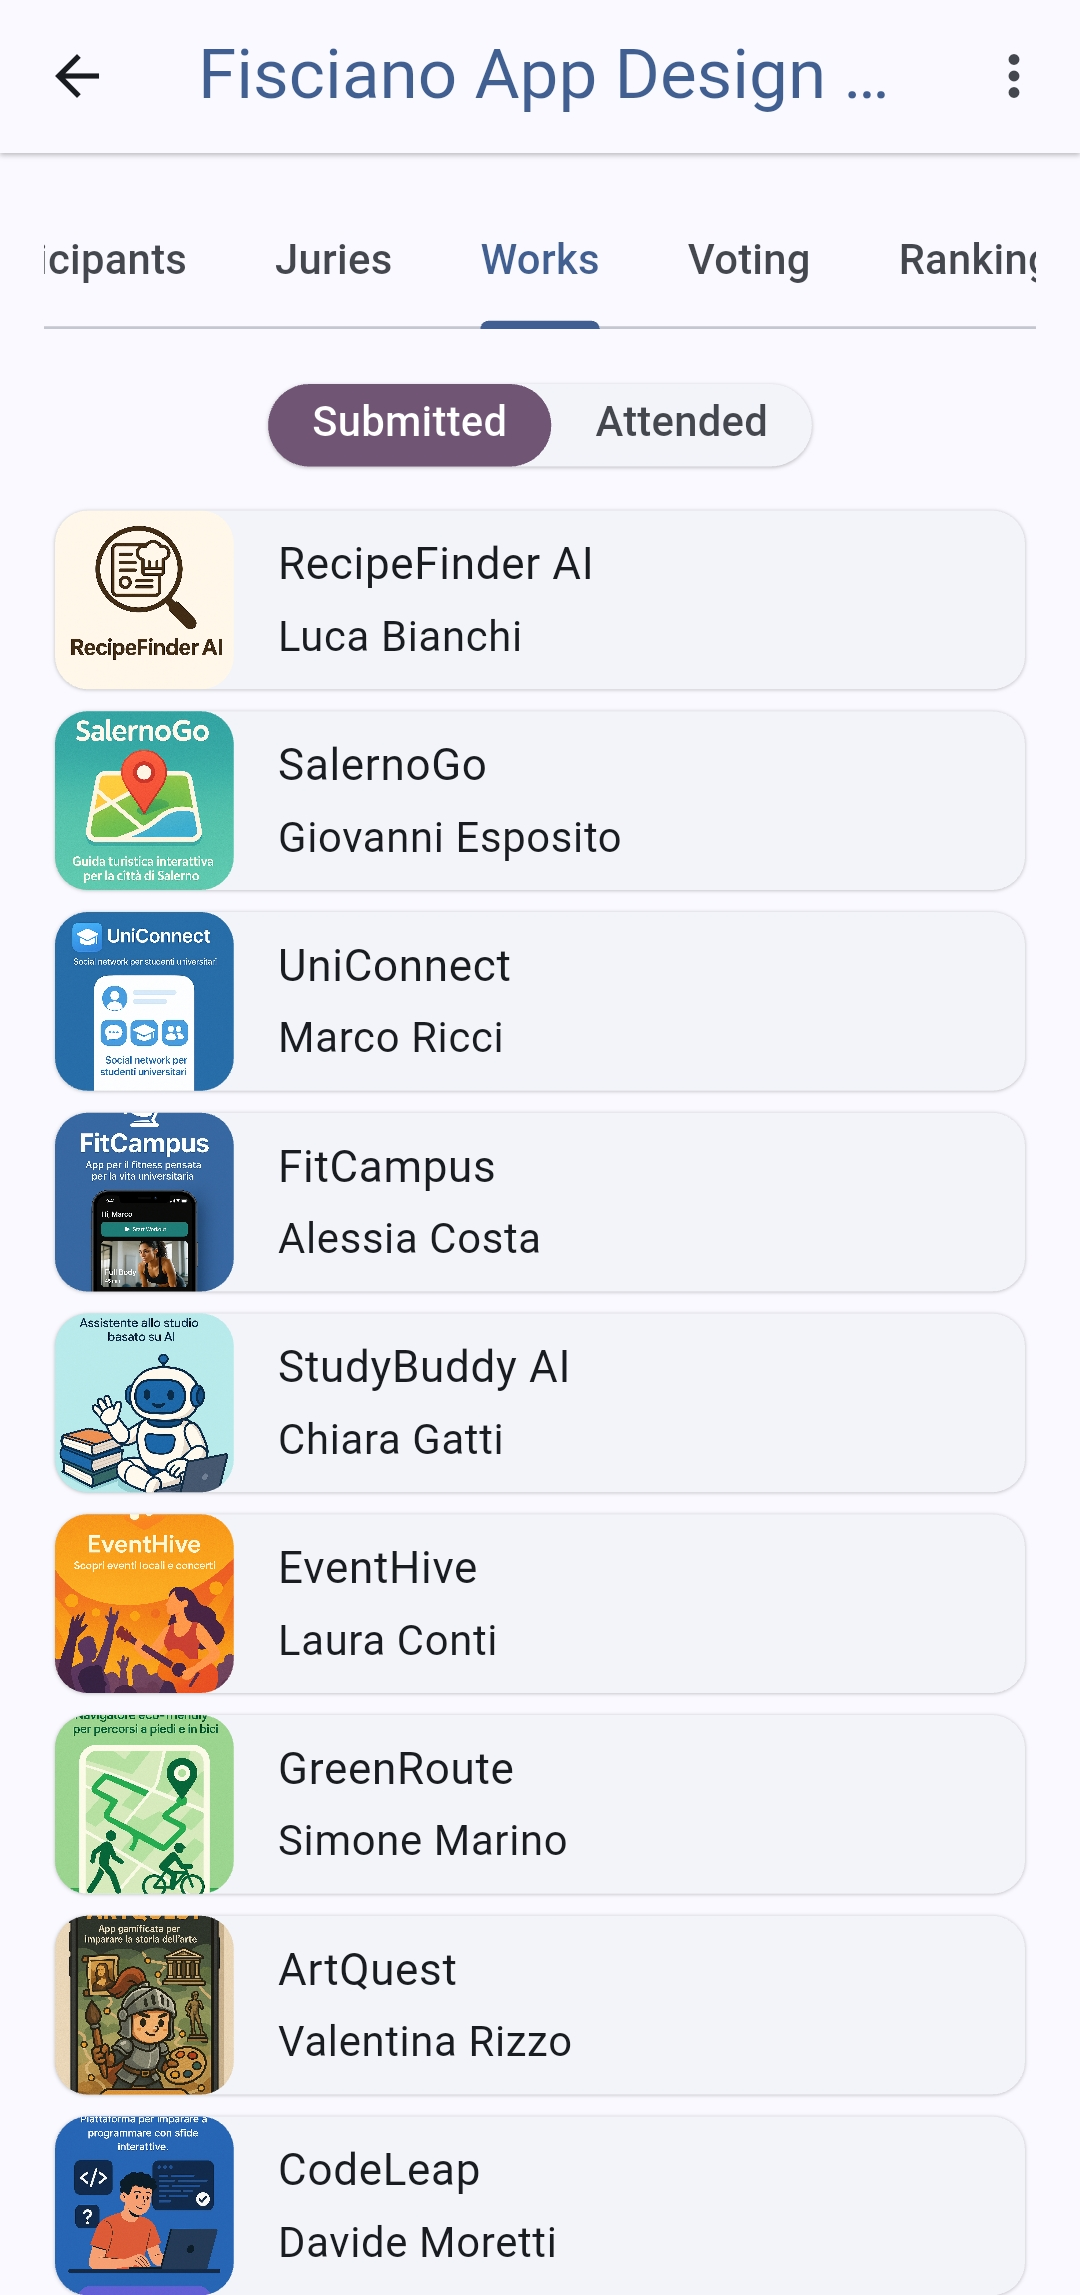
\includegraphics[width=\linewidth]{images/organizer-contest-works}
        \subcaption{Tab Works}
        \label{fig:contest_works}
    \end{minipage}
    \caption{Le principali tab di gestione all'interno di un contest.}
    \label{fig:contest_management_tabs}
\end{figure}

\paragraph{Terzo Flusso: Gestione della Sessione di Voto}
La tab \textbf{Voting} è dedicata alla gestione delle sessioni di voto.
Da qui, l'organizzatore può avviare una nuova sessione tramite un form a tre passaggi, dove può definire un nome per la sessione, selezionare i partecipanti da includere e, opzionalmente, impostare una restrizione geografica.
Una volta avviata, la schermata mostra lo stato \textbf{Live} della sessione, il token per i giurati semplici e permette di monitorarne l'andamento.

% --- FIGURE: Avvio Sessione di Voto (3+1 immagini) ---
\begin{figure}[H]
    \centering
    \begin{minipage}{0.32\textwidth}
        \centering
        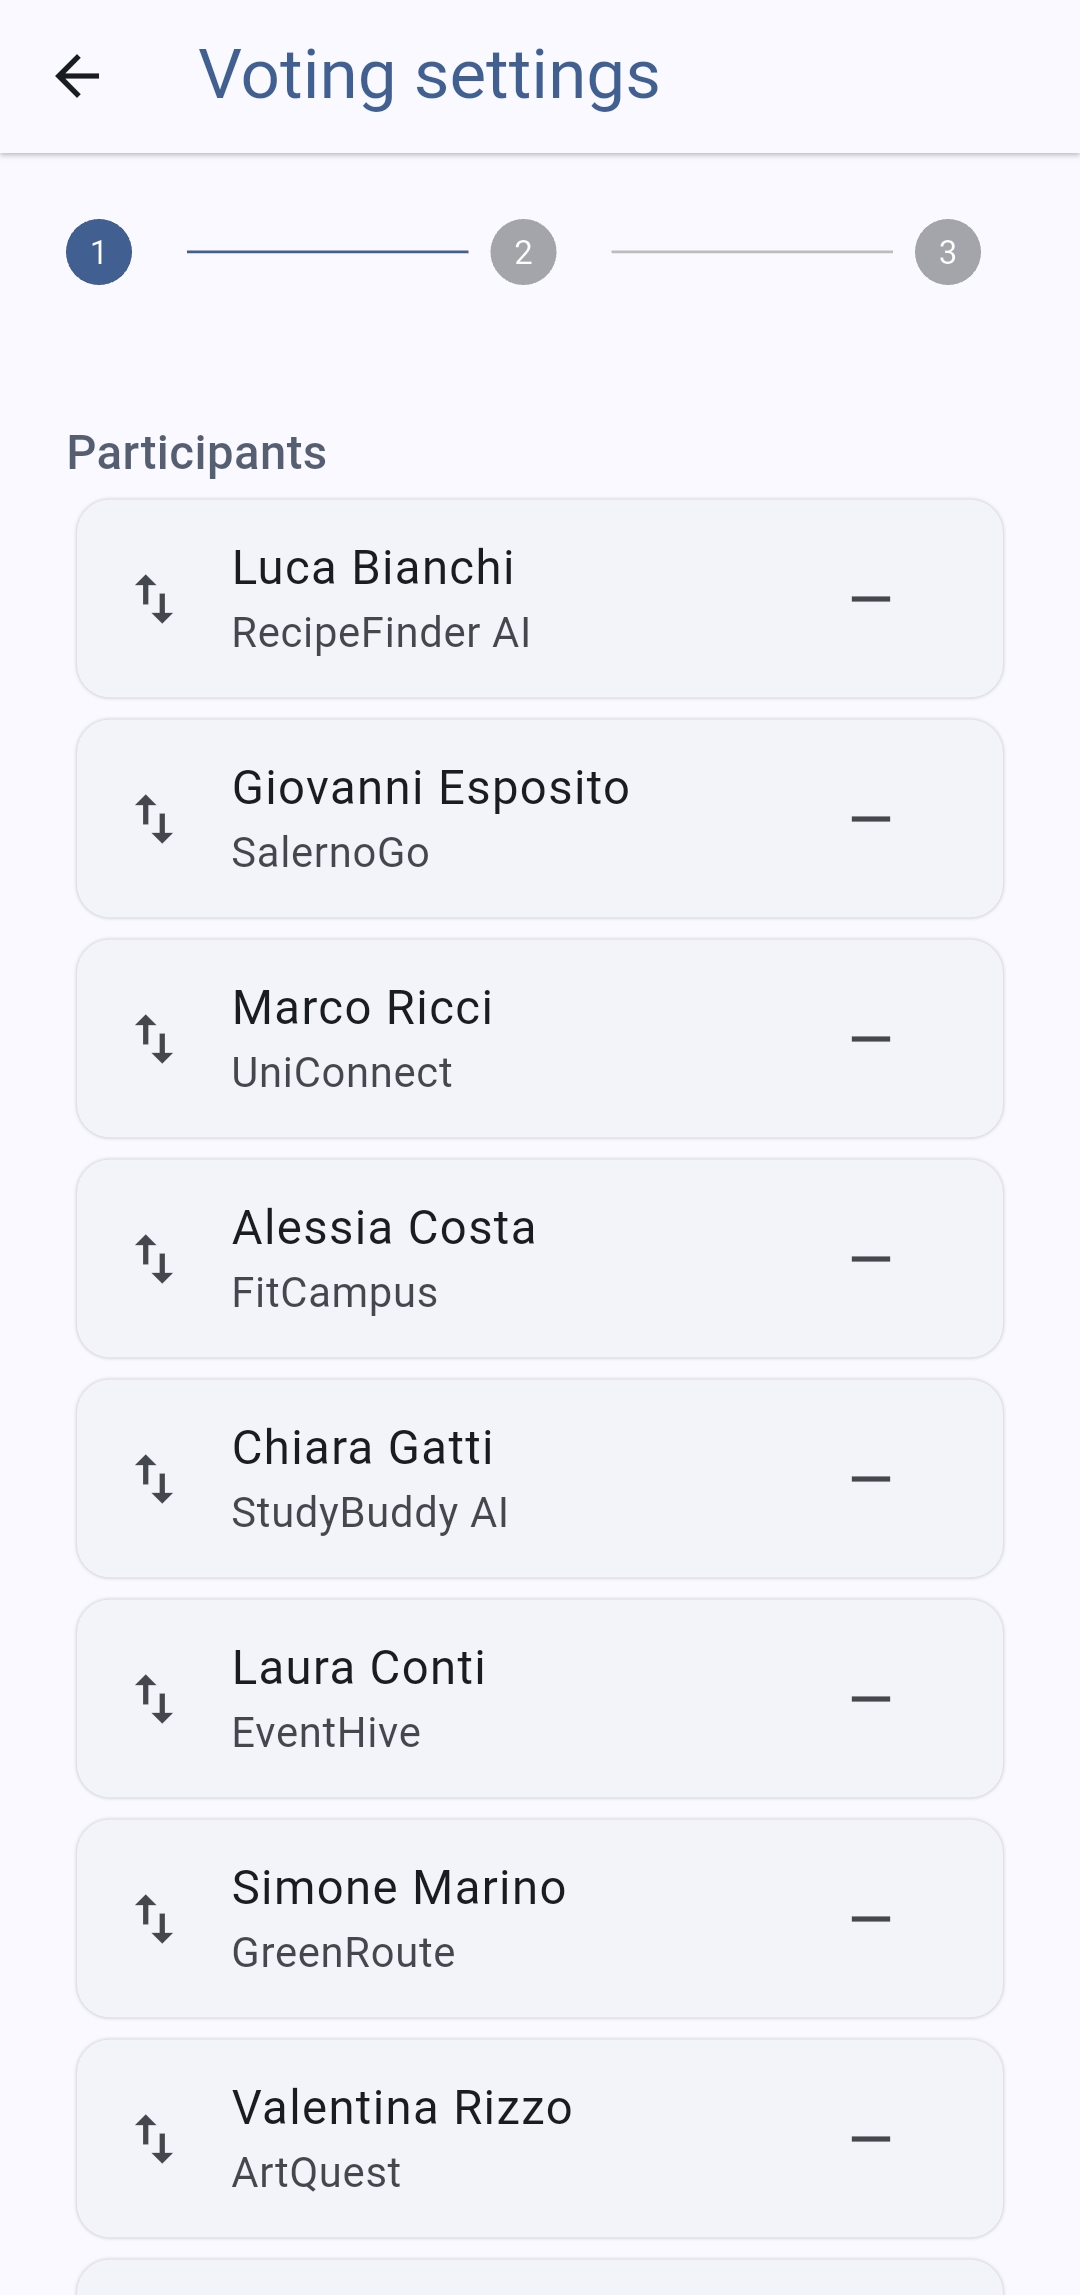
\includegraphics[width=\linewidth]{images/organizer-voting-session-step1}
        \subcaption{Passo 1: Info}
        \label{fig:voting_session_1}
    \end{minipage}\hfill
    \begin{minipage}{0.32\textwidth}
        \centering
        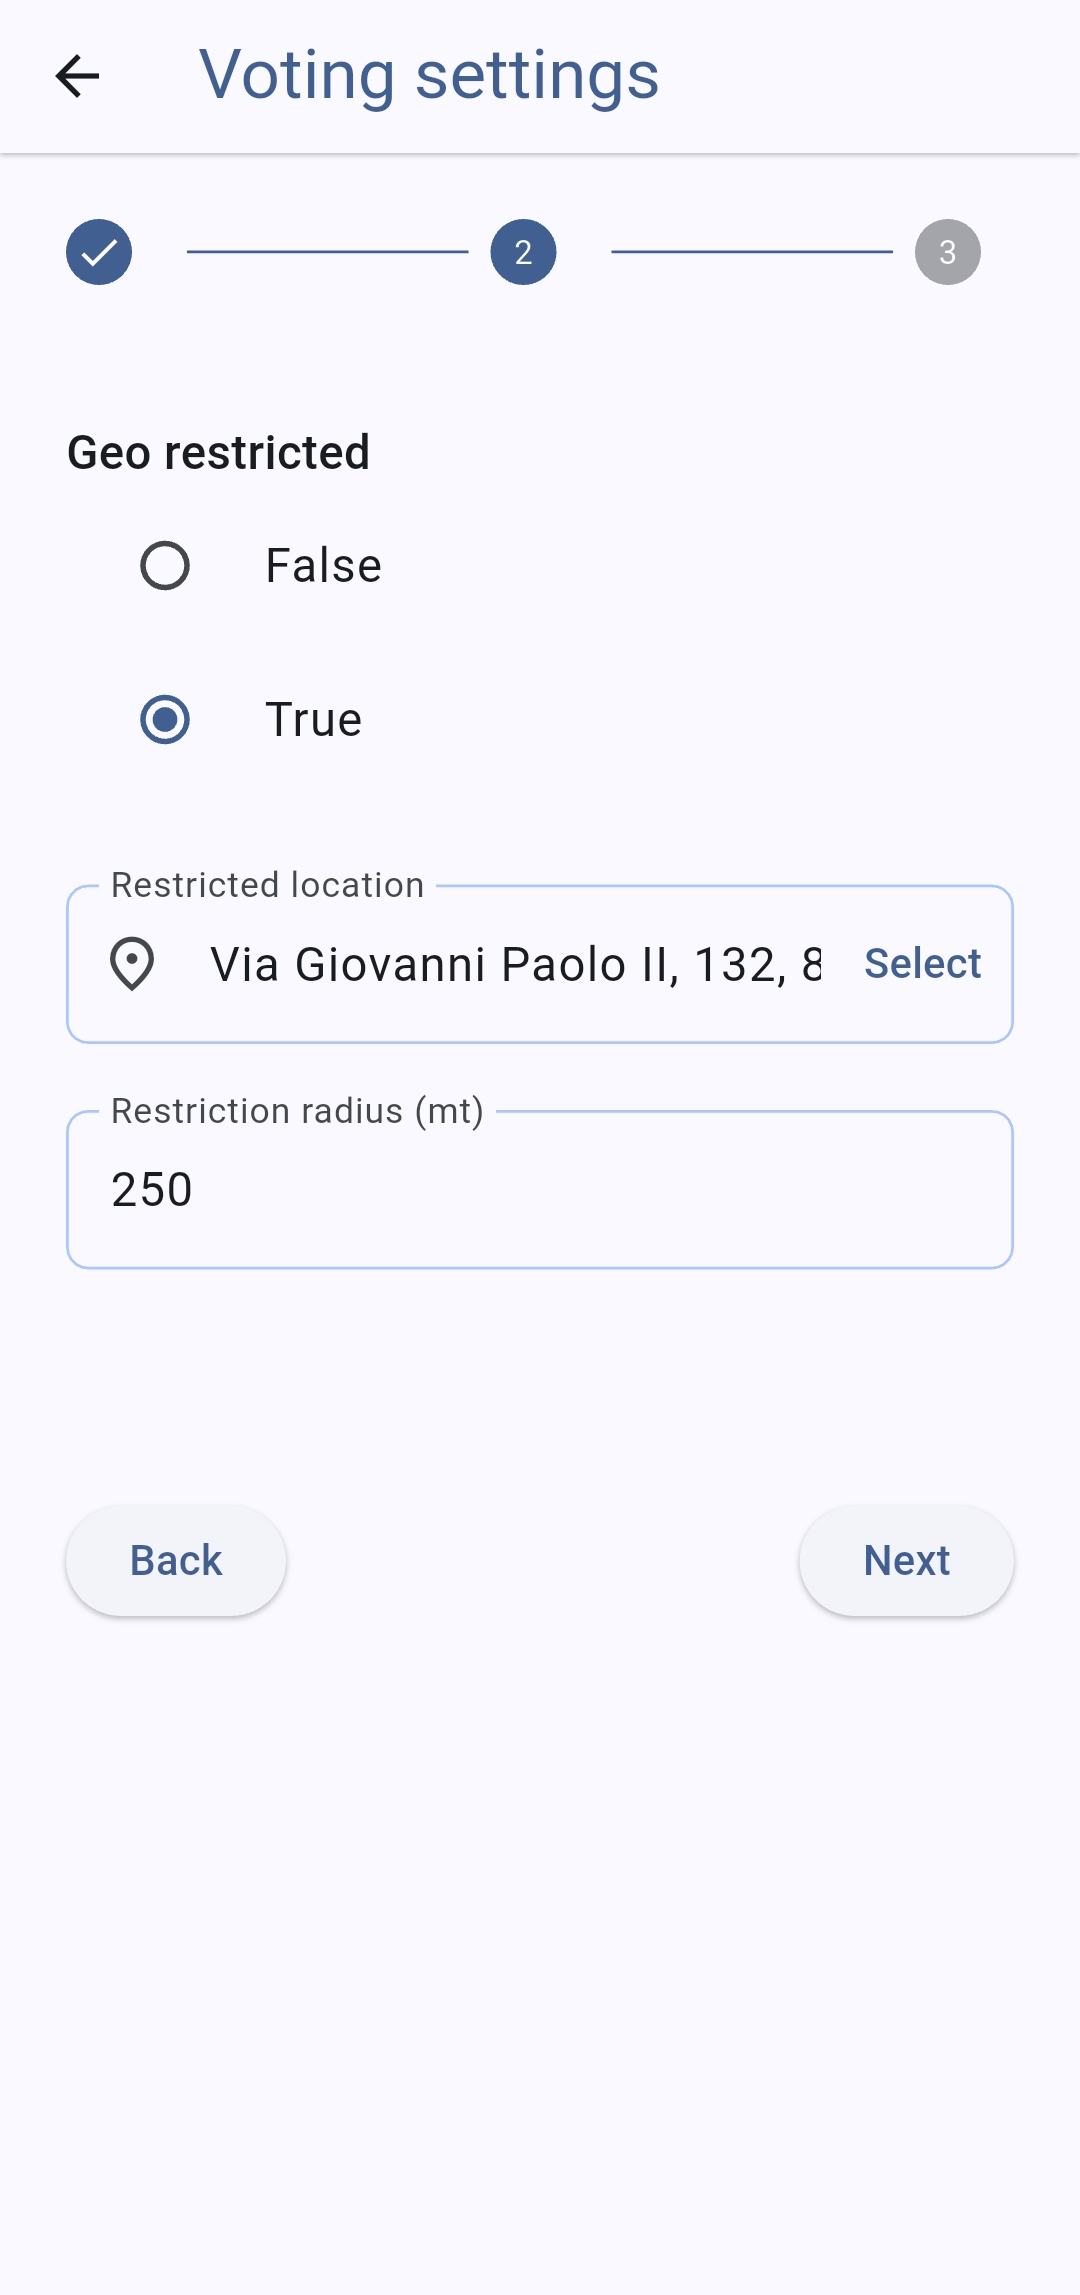
\includegraphics[width=\linewidth]{images/organizer-voting-session-step2}
        \subcaption{Passo 2: Partecipanti}
        \label{fig:voting_session_2}
    \end{minipage}\hfill
    \begin{minipage}{0.32\textwidth}
        \centering
        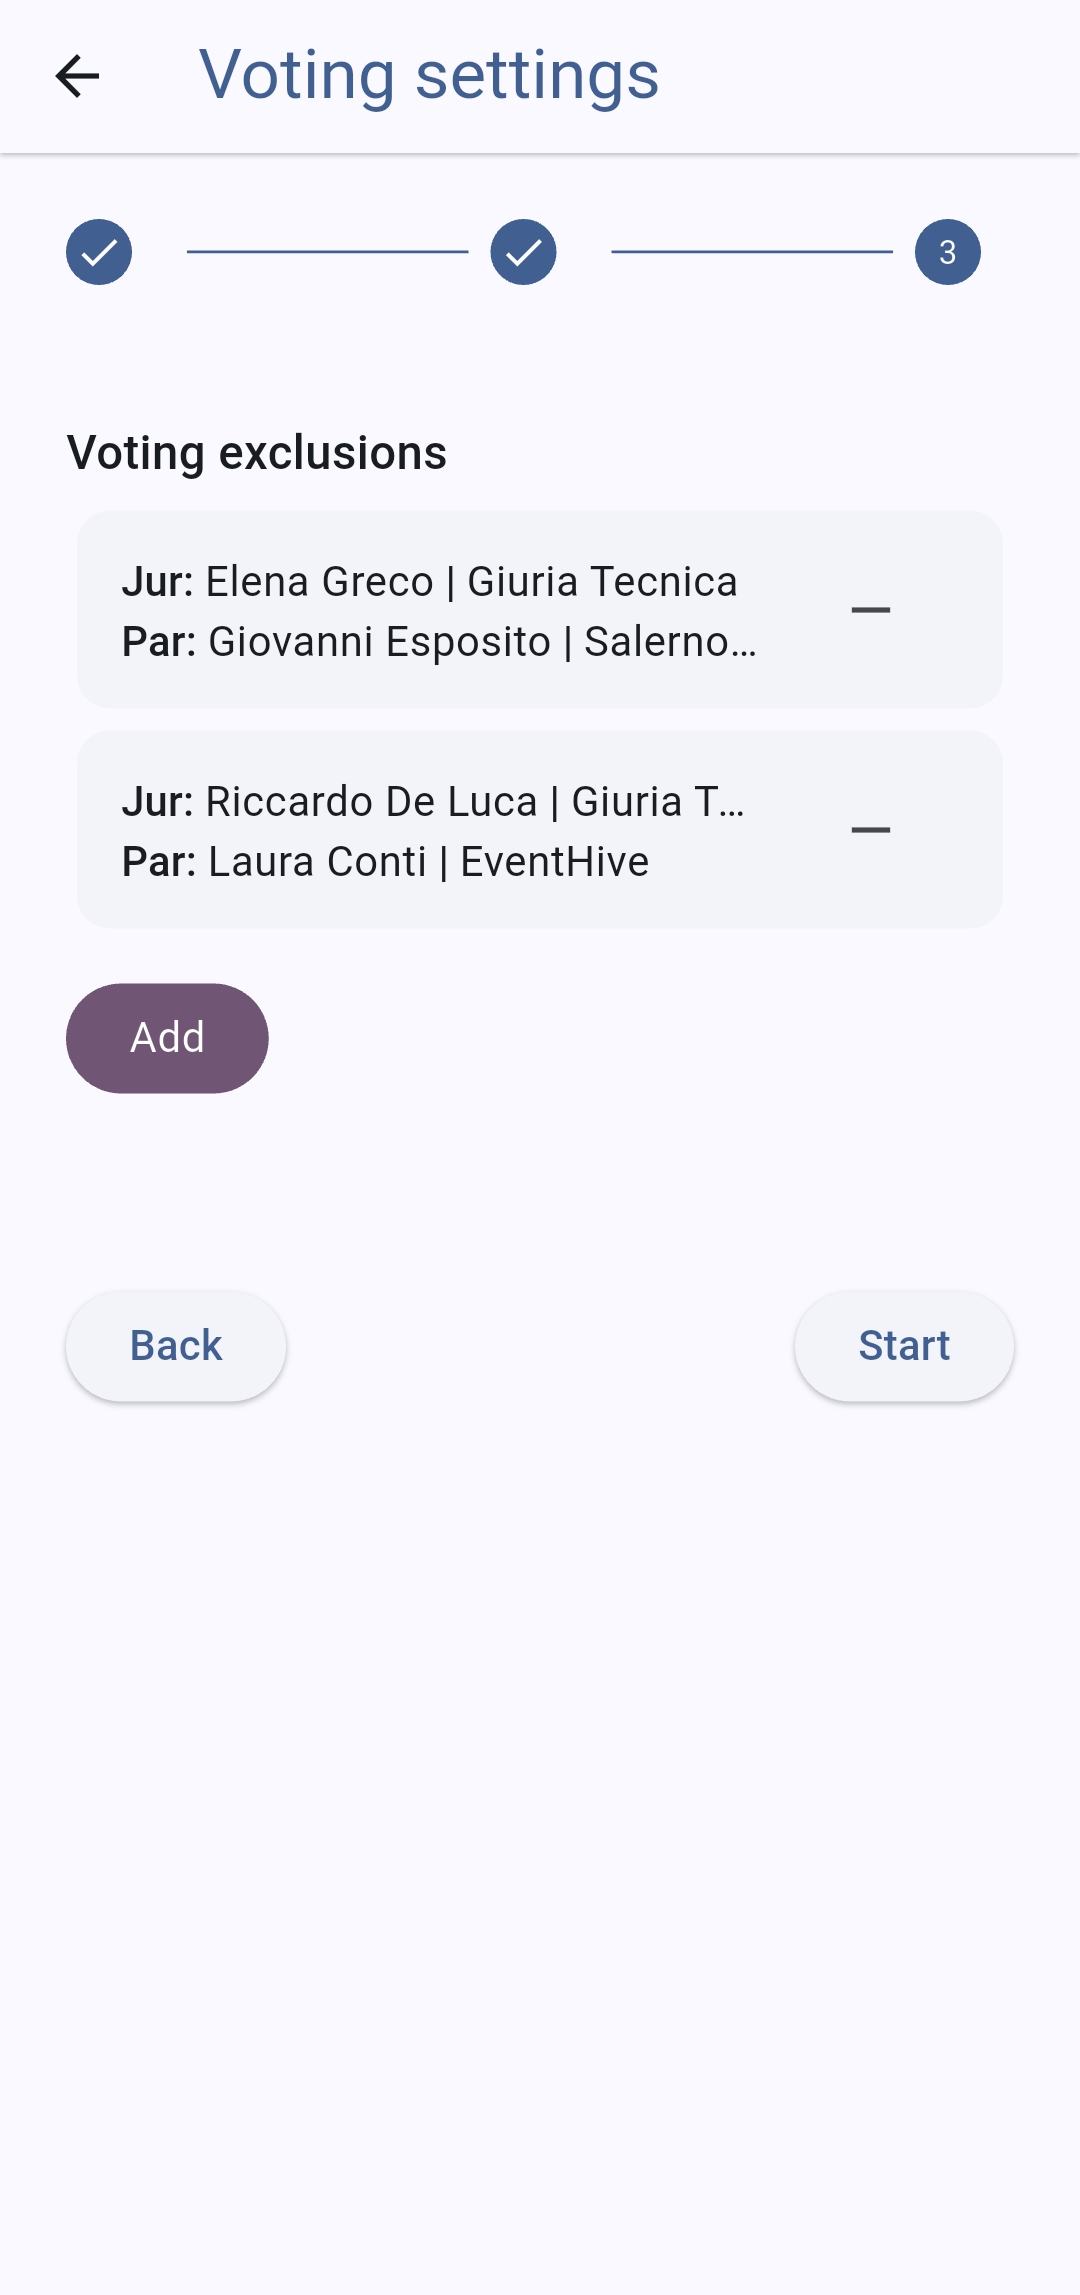
\includegraphics[width=\linewidth]{images/organizer-voting-session-step3}
        \subcaption{Passo 3: Geo-restrizione}
        \label{fig:voting_session_3}
    \end{minipage}
    \caption{I passaggi per la configurazione di una nuova sessione di voto.}
    \label{fig:voting-session-setup}
\end{figure}

\begin{figure}[H]
    \centering
    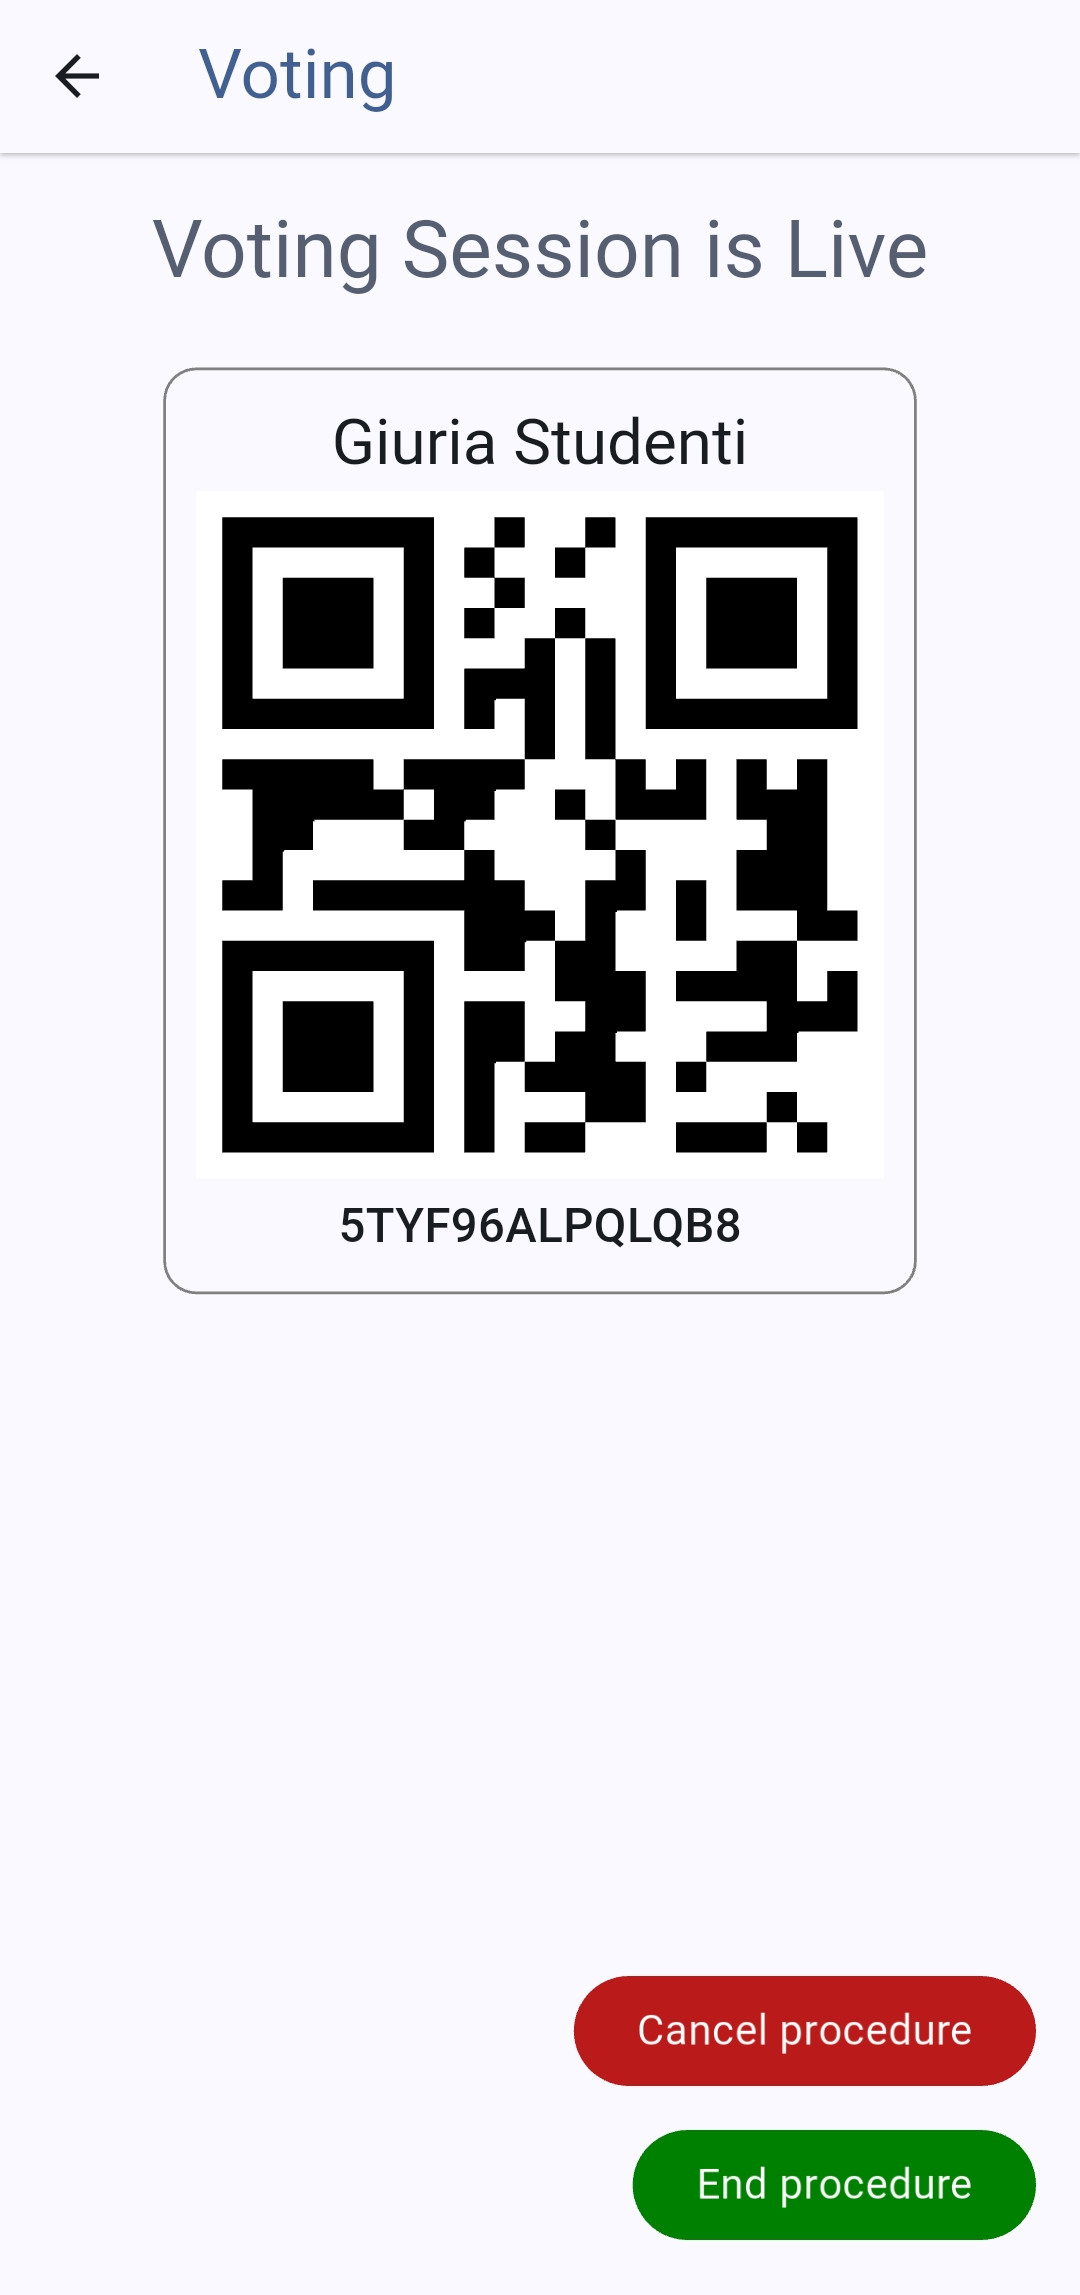
\includegraphics[width=0.5\textwidth]{images/organizer-voting-session-live}
    \caption{La schermata di una sessione di voto attiva (\emph{Live}).}
    \label{fig:voting-session-live}
\end{figure}

\paragraph{Quarto Flusso: Analisi dei Risultati e Classifiche}
Terminata la votazione, la tab \textbf{Results} permette all'organizzatore di analizzare i dati.
Può esplorare le \textbf{sottomissioni dei voti} di ciascun giurato, visualizzando le risposte fornite per ogni sezione del form (header, participant, footer).
Successivamente, può accedere alla sezione \textbf{Rankings}, dove può \textbf{generare una classifica} per una specifica giuria, selezionando i campi di tipo slider da includere nel calcolo.
La classifica generata viene mostrata in anteprima e può essere scaricata o pubblicata.

% --- FIGURE: Risultati e Classifiche (3+1 immagini) ---
\begin{figure}[H]
    \centering
    \begin{minipage}{0.32\textwidth}
        \centering
        
\includegraphics[width=\linewidth]{images/organizer-voting-results-header}
        \subcaption{Voti Header}
        \label{fig:results_header}
    \end{minipage}\hfill
    \begin{minipage}{0.32\textwidth}
        \centering
        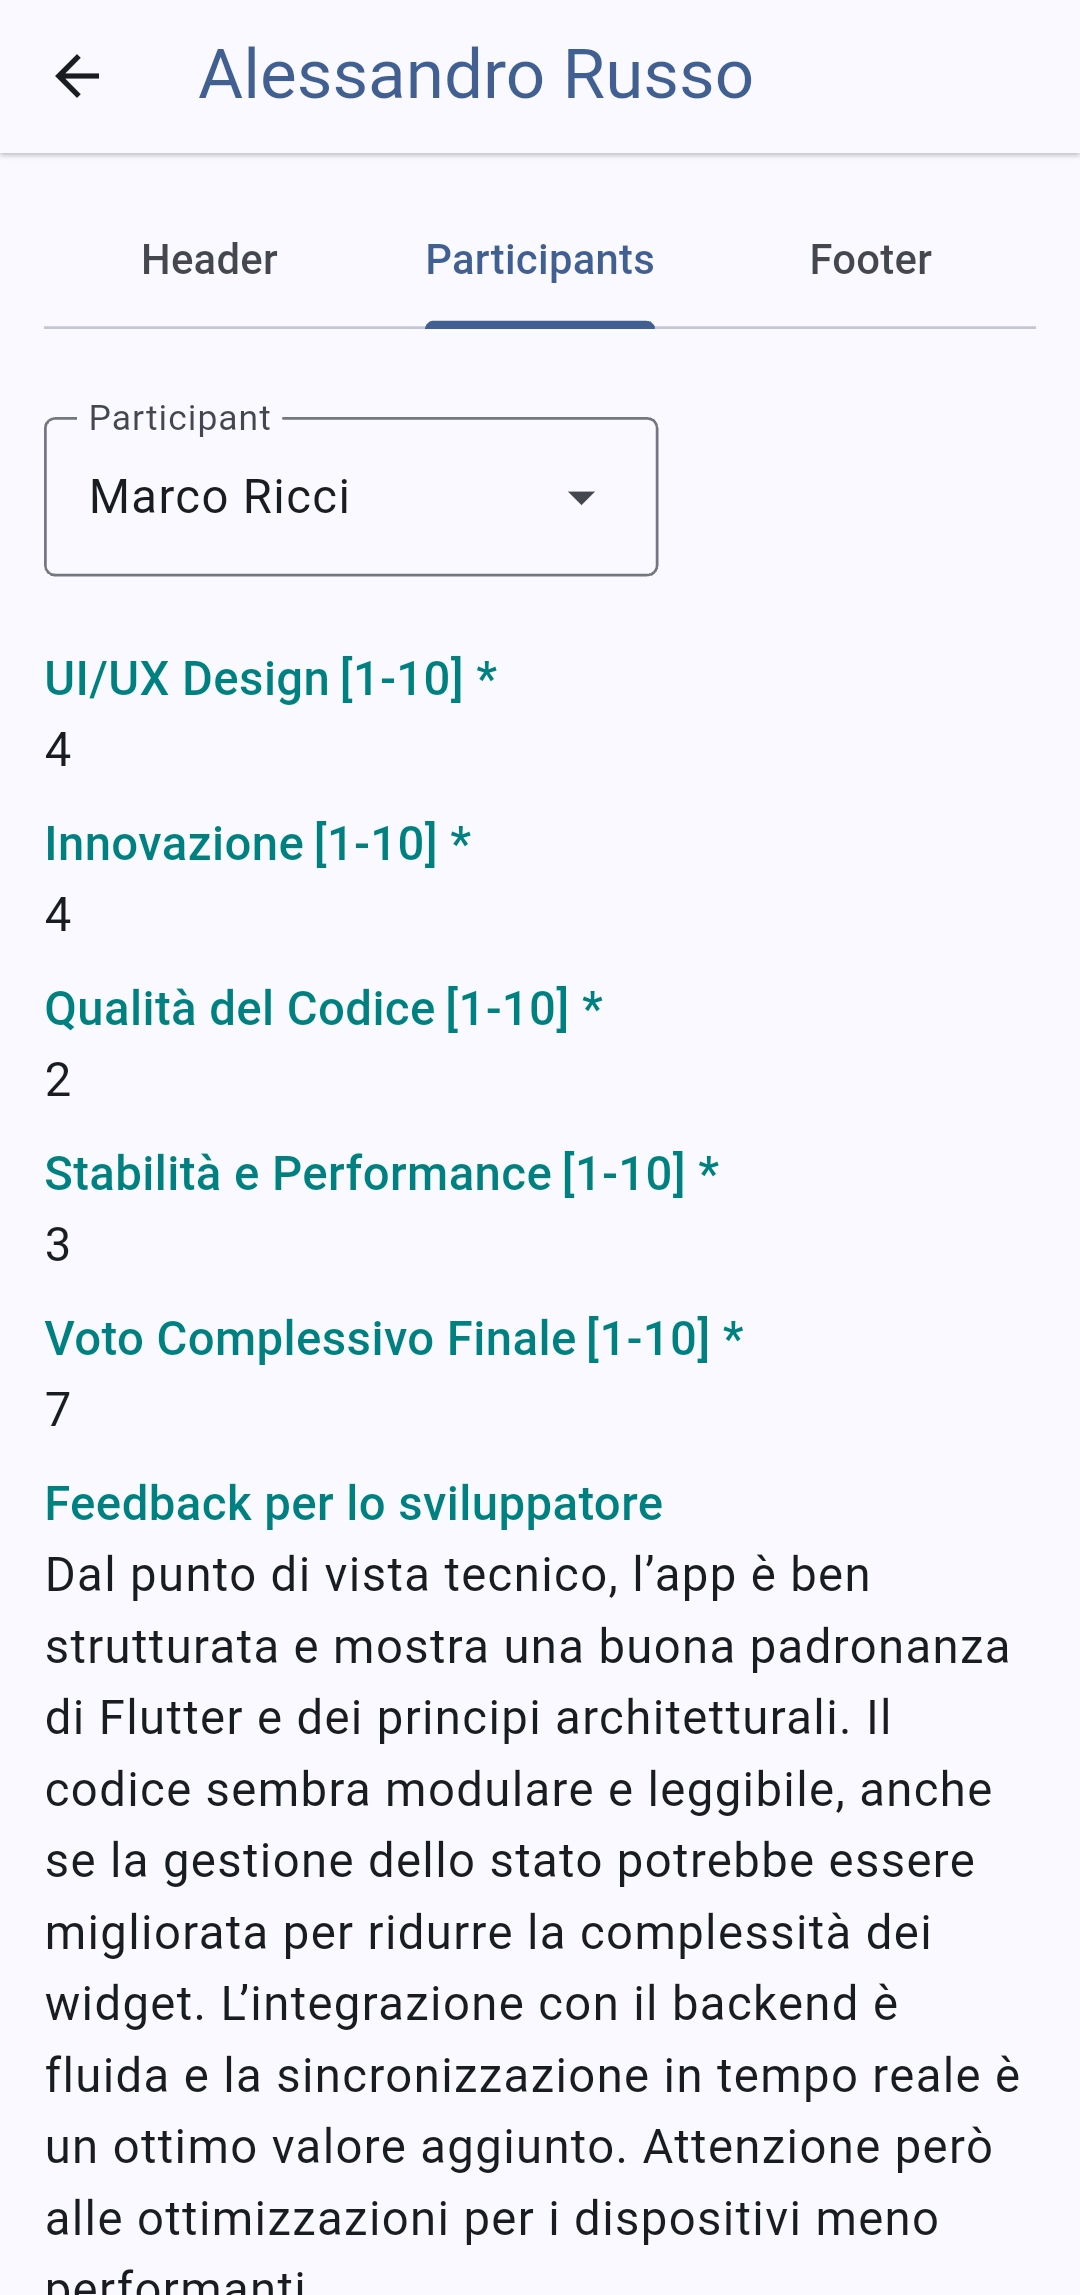
\includegraphics[width=\linewidth]{images/organizer-voting-results-participant}
        \subcaption{Voti Participant}
        \label{fig:results_participant}
    \end{minipage}\hfill
    \begin{minipage}{0.32\textwidth}
        \centering
        
\includegraphics[width=\linewidth]{images/organizer-voting-results-footer}
        \subcaption{Voti Footer}
        \label{fig:results_footer}
    \end{minipage}
    \caption{Visualizzazione dei voti inviati da un giurato, suddivisi per scope.}
    \label{fig:results-submission-view}
\end{figure}

\begin{figure}[H]
    \centering
    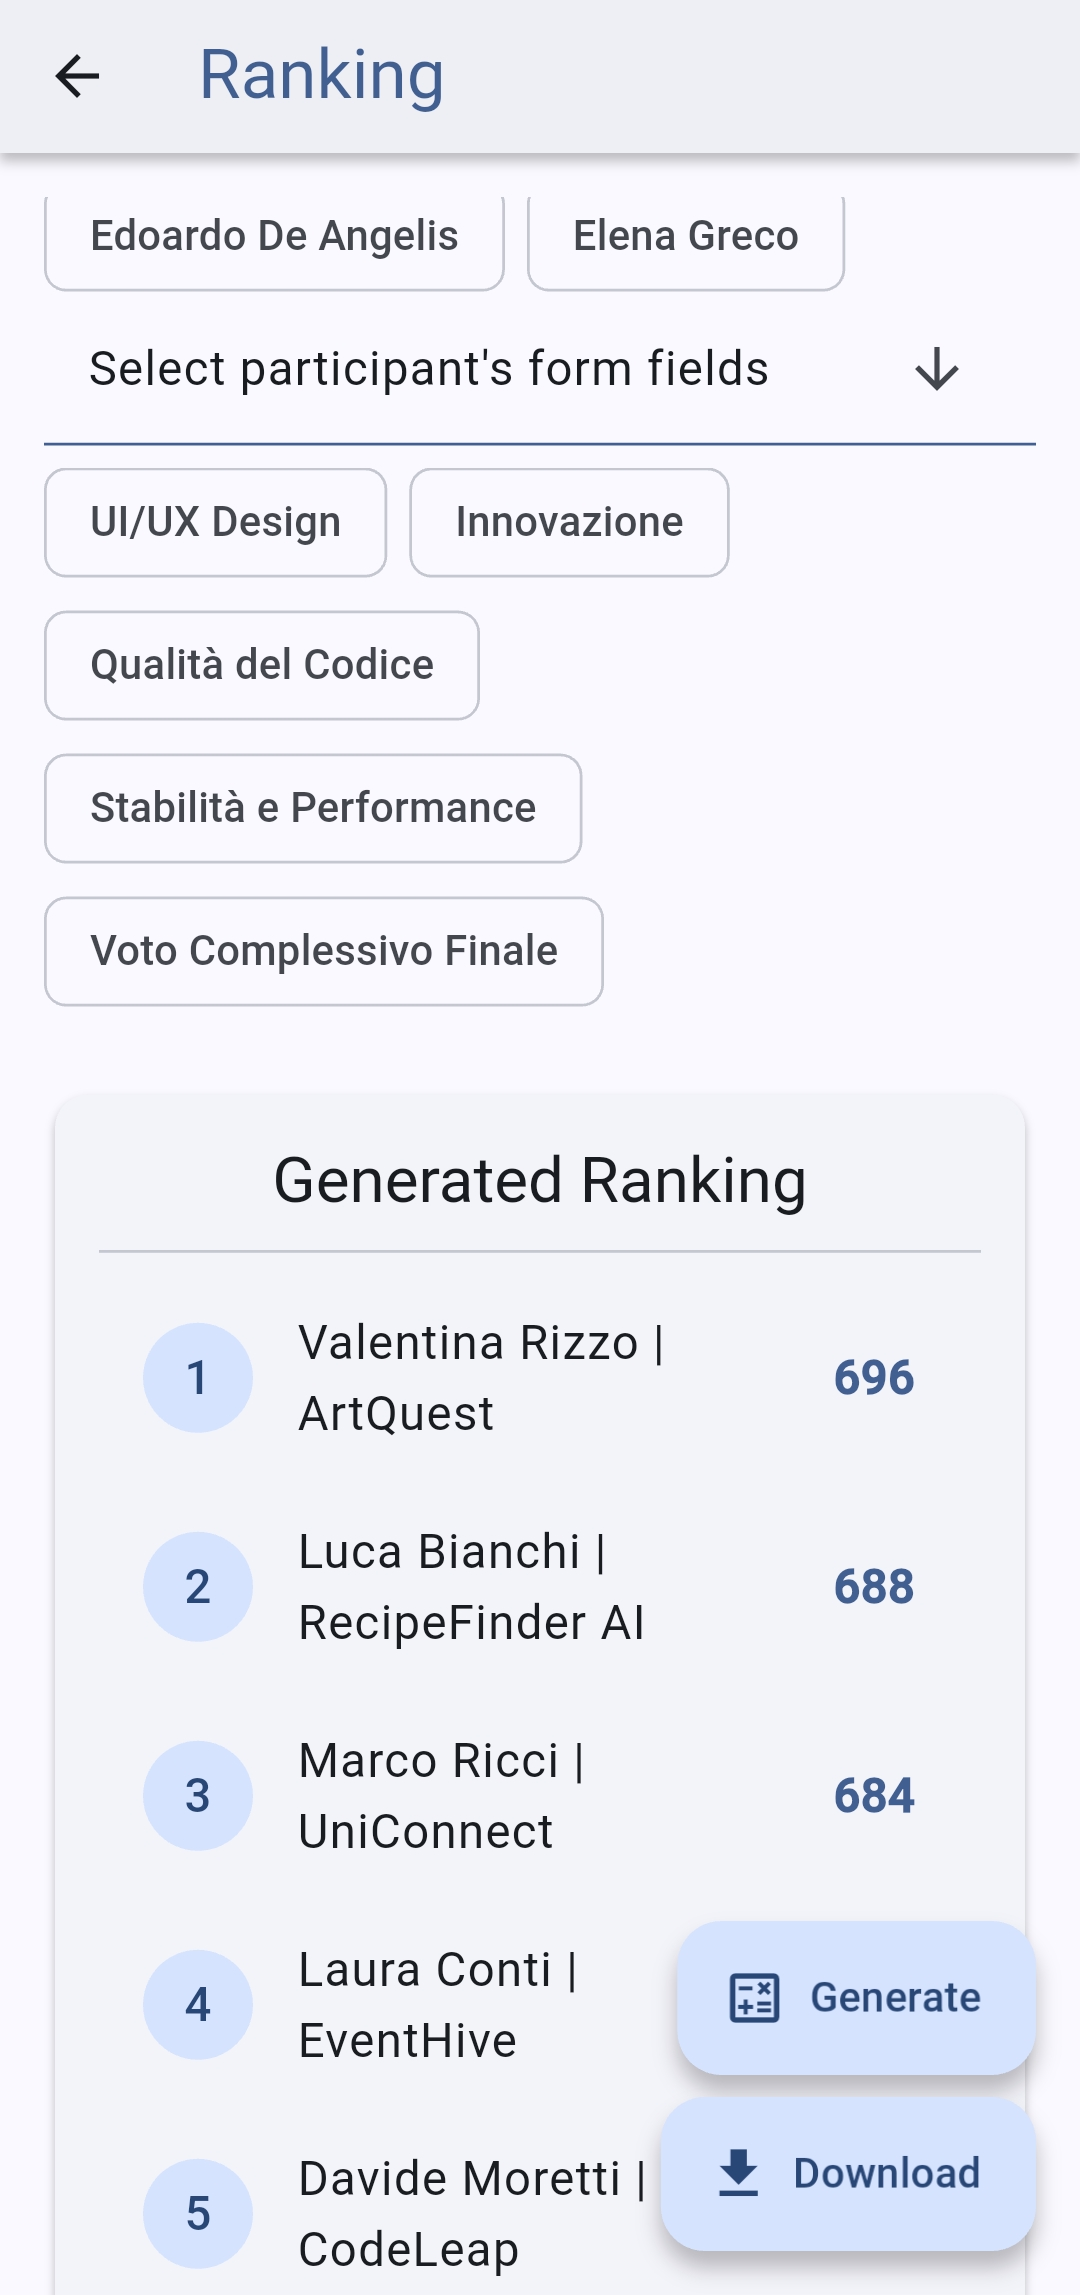
\includegraphics[width=0.5\textwidth]{images/organizer-ranking-generation}
    \caption{La pagina per la generazione della classifica di una giuria.}
    \label{fig:ranking-generation}
\end{figure}






%\section{Prodotto finale: Flussi Operativi e Interfaccia Utente}\label{sec:prodotto-finale:-flussi-operativi-e-interfaccia-utente}
%Il prodotto finale offre interfacce e flussi operativi specifici e ottimizzati per ogni attore del sistema, garantendo un'esperienza utente coerente tra la versione web e quella Android.
%Le sezioni seguenti descrivono il ciclo di vita completo di un contest attraverso i percorsi dei suoi protagonisti.
%
%\subsection{Flusso dell'Organizzatore}\label{subsec:flusso-dell'organizzatore}
%L'organizzatore è l'utente con il set di funzionalità più ricco, responsabile dell'intero ciclo di vita del contest.
%
%\paragraph{Creazione e Configurazione}
%Dopo l'autenticazione, l'organizzatore accede a una dashboard personale dove può visualizzare e gestire i contest da lui creati.
%Il flusso principale lo guida attraverso la creazione di un nuovo contest tramite un form multi-step in cui inserisce dati principali (nome, descrizione, data), periodo di sottomissione, luogo e immagini rappresentative.
%Una volta creato il contest, accede a un pannello di gestione dettagliato dove può:
%\begin{itemize}
%	\item \textbf{Creare le giurie}, specificando se sono di tipo \emph{appointed} (per giurati nominati) o \emph{simple} (per giurati semplici con token).
%	\item \textbf{Invitare i partecipanti e i giurati nominati}, inserendo i loro indirizzi email.
%	Apposite Edge Functions gestiscono l'invio sicuro delle email di invito.
%	\item \textbf{Configurare il form di voto} associato a ciascuna giuria, definendo i campi testuali e slider con i relativi scope (header, participant, footer).
%\end{itemize}
%
%% TODO FIGURA: Inserire qui uno screenshot della dashboard dell'organizzatore con l'elenco dei suoi contest.
%% TODO FIGURA: Inserire qui uno screenshot della pagina di configurazione di un VotingForm.
%
%\paragraph{Gestione della Votazione e dei Risultati}
%Terminato il periodo di sottomissione, l'organizzatore avvia una \emph{VotingSession}, creando lo snapshot immutabile dei dati.
%Una volta che tutti i giurati hanno votato, chiude la sessione.
%Ora ha a disposizione i risultati per ciascuna giuria, che può esportare in formato Excel (xlsx).
%Ha inoltre la possibilità di generare una classifica per ciascuna giuria selezionando i campi required, di tipo slider, e con scope participant, che desidera considerare.
%La classifica viene visualizzata in app e può essere scaricata in formato PDF\@.
%A questo punto l'organizzatore può raffinare le classifiche esternamente, ad esempio può generare un'unica classifica considerando quelle di tutte le giurie, e pubblicarla in formato pdf, rendendola disponibile per il download per i partecipanti e giurati nominati facenti parte del contest.
%%Durante la sessione, può monitorarne l'andamento in tempo reale.
%
%% TODO FIGURA: Inserire qui uno screenshot della pagina di monitoraggio di una sessione di voto.
%
%\subsection{Flusso del Partecipante}\label{subsec:flusso-del-partecipante}
%Il partecipante, una volta accettato l'invito a un concorso, ha un percorso chiaro e focalizzato.
%La sua azione principale è la \textbf{sottomissione del proprio \emph{Work}}.
%Un form dedicato lo guida nel caricamento di un pacchetto \texttt{.zip} contenente il materiale principale e delle immagini di anteprima, che verranno usate durante la votazione.
%Al termine del concorso, può accedere alla sezione dei risultati per visualizzare la classifica finale, se pubblicata dall'organizzatore.
%
%% TODO FIGURA: Inserire qui uno screenshot della pagina di sottomissione del Work.
%
%\subsection{Flusso del Giurato (Nominato e Semplice)}\label{subsec:flusso-del-giurato-(nominato-e-semplice)}
%Il sistema supporta due modalità di accesso per i giurati, garantendo flessibilità.
%\begin{itemize}
%	\item Il \textbf{giurato nominato (\emph{appointed})} accede alla sua dashboard personale e visualizza l'elenco dei contest a cui è stato assegnato.
%	\item Il \textbf{giurato semplice (\emph{simple juror})}, invece, accede direttamente alla procedura di voto tramite un token fornito dall'organizzatore, senza bisogno di un account.
%\end{itemize}
%Per entrambi, l'interfaccia di voto è identica e li guida attraverso una procedura strutturata: per ogni \emph{Work} in gara, viene presentato il materiale di anteprima e il \emph{VotingForm} da compilare.
%Il sistema garantisce che i voti possano essere inviati una sola volta per sessione.
%
%% TODO FIGURA: Inserire qui uno screenshot della procedura di voto del giurato, evidenziando la visualizzazione di un'opera e la compilazione di un campo slider.
%
%\subsection{Flusso delle Notifiche}\label{subsec:flusso-delle-notifiche}
%Per mantenere tutti gli utenti informati, il sistema include una \textbf{inbox} interna, accessibile dalla barra di navigazione principale.
%Qui, tutti gli utenti autenticati ricevono notifiche generate automaticamente per eventi rilevanti, come la ricezione di un invito, la cancellazione di un contest o la pubblicazione di una classifica.
%La ricezione di nuovi messaggi avviene in tempo reale, segnalata da un indicatore visivo sull'icona della inbox, grazie all'integrazione con il servizio Realtime di Supabase.
%
%% TODO FIGURA: Inserire qui uno screenshot della pagina Inbox con un elenco di messaggi di notifica.

